\documentclass[a4paper,11pt]{report}
\usepackage[T1]{fontenc}
\usepackage[english]{babel}
\usepackage{fancyhdr}
\usepackage{hyperref}
\usepackage{graphicx}
\usepackage{float}
\usepackage{wrapfig}
\usepackage{listings}
\usepackage[usenames, dvipsnames]{color}
\usepackage{longtable}
\usepackage{fontawesome}

\setlength{\textwidth}{16cm}
\setlength{\textheight}{24cm}
\setlength{\oddsidemargin}{0cm}
\setlength{\voffset}{-2.2cm}
\setlength{\headheight}{15pt}
\setlength{\parindent}{0pt}
% Disables red links
\hypersetup{pdfborder={0 0 0}}

\pagestyle{fancy}
\lhead{\small\textsc{GeoTwit - Thesis}}
\rhead{\small\textsc{Miguel Santamaria -- \today}}

\title{GeoTwit - Thesis}
\author{Miguel Santamaria}
\date{\today}

% MIGUEL TODO: rechercher '–', '“', '”' et '’'.
% MIGUEL TODO: miniscules aux "\caption"
% MIGUEL TODO: Tweet -> tweet
% MIGUEL TODO: Pas "GeoTweet", mais "GeoTwit"

\begin{document}
\maketitle

% Hide header and footer
% MIGUEL TODO: mettre le nombre de pages
\thispagestyle{empty}
\vspace*{8cm}
\begin{center}
    \textbf{Acknowledgement}\\
    \bigskip
    I would first like to thank my thesis supervisor, 
    %MIGUEL TODO
\end{center}

\setcounter{page}{0}

% MIGUEL TODO
\chapter*{Abstract}
The purpose of this project is to enable analysis of varied subjects using the social platform of \emph{Twitter}, static or in real-time, using an application that provides an expanded geographic filtering of tweets and generates maps and charts on the analysis, \emph{GeoTwit}. This paper thus contains the analysis, development and implementation of this web tool, as well as numerous and varied subjects that have already been analysed over the duration of a semester, at the level of individual topics as well as current events.\\
In preparation for the development of this tool, market studies were realized in addition to a thorough analysis of different Twitter's APIs, in order to glean the most optimal approach for the project. Furthermore, several prototype applications were developed and tested in advance, to understand and resolve the potential roadblocks and issues that could and did arise in the course of development. Finally, various schemas and diagrams like the mock-up and UML schemas were prepared, in order to visualize and discretize the steps involved. The final implementation integrates and streamlines all these tools to allow the end user to analyze a maximum of two simultaneous subjects in real-time. Static analyses are also possible, but are not as expanded as the real-time functionality. Requiring the user to connect to his Twitter account, the application allows him/her to import and export their analyses (maps, charts, speed reception and various other useful information) as external files.

\tableofcontents
\newpage
\thispagestyle{empty}
~
\newpage

\chapter{Introduction}
% MIGUEL TODO
\section{Summary of the Problem}
Within the span of a few years, social networks have rapidly mushroomed across the globe to become all encompassing and omnipresent in our lives. Across such networks, a massive quantity of data is shared at every moment in time, and each time a larger volume from the preceding day. In addition to a widespread use by lambda people, the scientific community has been finding novel ways to analyse and make sense of this cascade of available social information: \emph{data mining}. Indeed, what better source there is than a social network, continuously and increasingly reporting collective human opinion and behaviour in real-time, to analyse human-oriented subjects?\\\\
The goal of this project is thus to set up a web application that allows users to enter one or two subjects of their choice, to visualize a real-time activity graph/map for these subjects both on Twitter and on a geographic map and finally to import and export the results as external files. Static analyses are also possible, but are not as expanded as the real-time functionality.
\bigskip

\section{Generalities}
This project - \emph{GeoTwit} - is carried out as the final Bachelor thesis within the TIC department of the Computer Engineering sector of the Yverdon-les-Bains's HEIG-VD school, for the IICT institute. The student - \emph{Miguel Santamaria} - supported by his supervisor - \emph{Ph.D. Nastaran Fatemi}, professor and teacher - worked alone on his project, at the level of both development and documentation. Note that this project is not confidential.\\\\
The project - selected in \emph{December 2015} and started on \emph{February 22, 2016} - covers several different aspects of web development as well as intelligent analysis (data mining) and data visualization. A progress report was asked for the \emph{June 17, 2016}, the final thesis was delivered on \emph{July 29, 2016}, and the oral defense is planed for the \emph{September 5, 2016}. The basic duration of the project is \emph{450 hours}, even if the work was done in less time than this value.
\bigskip

\section{Specifications}
\subsubsection{Functionalities}
The application provides the following features:
\begin{itemize}
	\item The reading of keywords and the selection of geographic areas on the map by the user.
	\item The retrieval of tweets, using the Twitter's APIs.
		Note that only a certain percentage of these tweets include geographic information, necessary for the future operations; a first filtering is thus operated here.
	\item The analysis and the filtering of tweets via calculation of the number of tweets by areas and by subjects.
	\item The visualization of the results on maps.
	\item The interaction (zoom-in, zoom-out, etc.) with the maps. The development of this feature involved the use of appropriate algorithms (like tweet grouping) and libraries.
	\item The generation of data charts and the possibility to import/export one's analysis.
\end{itemize}

\subsubsection{Used Technologies}
The suggested tools for this project were the \emph{Scala} language coupled with \emph{Play Framework}, while noting other technological choices were also possible. Due to both the personal interests of the student and a certain curiosity for unknown technologies in general, it was decided that these choices will be retained.
Lacking proficiency in either of these technologies, the student was initially required to learn the Scala language and the use of Play Framework before starting the development on the application.
Note that the \emph{JavaScript} web language is used to complement the client side of the application.

\chapter{Analyses}
This chapter contains all the analyses done before the implementation of the application itself.

\section{Existing Applications / Market Studies}
There are several existing applications that allow a user to visualize tweets on a map, the most visible being:
\begin{itemize}
	\item \textbf{One Million tweet Map}\footnote{http://onemilliontweetmap.com/}: the One Million tweet Map application lays out, to some extent, what has been implemented in this project, i.e. displaying tweets in real time (filtered or not) on a geographical map with grouping methods.\\\\
	However, unlike GeoTwit, the application does not offer a static search and view of tweets nor the possibility to export and import the analyzed data and to access and analyze charts. In addition, it also does not offer the possibility to analyze and compare two subjects at the same time or to filter tweets by language or location of the tweet. Nevertheless, this application does not require users to connect with their Twitter's accounts, for using the application.
	\item \textbf{TrendsMap}\footnote{http://trendsmap.com/ - found via mashable.com/}: this application shows a real-time mapping of Twitter trends across the world. If you click on any word you will see a real-time stream of relevant tweets. One must register and/or pay for further access to features/content.\\\\
	The interesting feature of this application is the display of current trends across the world, which is not currently present in GeoTwit. Users are also not required to connect to their Twitter accounts. However, users have to pay to access more detailed content, and there is no possibility to access static content nor to filter tweets with more complex filters or to access data analysis and visualization tools like charts. There is also not the possibility of importing and exporting one's analysis report.
	\item \textbf{tweetping}\footnote{https://tweetping.net/}: shows real-time reception of tweets all around the world on a map.\\\\
	Since the application is still in a beta phase, it is not possible to access most features, but the application intends to offer data analysis tools like charts as well as a complex filtering process, nearly matching the GeoTwit's features. However as with the previous two apps, users do not seem to be able to access static features or import and export analysis. Users also need to pay in order to access more interesting functionalities, but don't have to connect with their Twitter accounts. A feature of note was that the GUI of this application is well designed and user friendly.
	\item \textbf{tweetMap}\footnote{https://worldmap.harvard.edu/tweetmap/}: This tool allows one to visualize tweets written in a certain period, and create interesting charts and visualizations.\\\\
	This application provides interesting tools to analyze static content with a map (complex filters and charts), perhaps more so than GeoTwit. Users also do not need to connect. In this case as well, there was not the possibility to analyze real-time data or export analysis.
	\item \textbf{Stweet}\footnote{http://tweet.we-love-the.net/Stweet/ found via mashable.com/}: his service combines Twitter and Google Street View data to provide us a location-based breakdown of trending topics in a specific neighborhood.\\\\
	This application, despite its simplicity, is innovative given the functionality of allowing the user to display tweets directly onto 3D street view.
	\item \textbf{GeoChirp}\footnote{http://tweet.geochirp.com/}: this app allows the user to search for tweets in a given location, but only in a static way (no real time updating).\\\\
This application is a basic one, only returning tweets in a given location, with the upper limit specified by the user. Like GeoTwit, users must connect to their Twitter's accounts to use the application. However, there is no way to analyze real-time data or visualize the data.
	\item \textbf{tweet To Map}\footnote{http://tweettomap.com/}: this web plug-in allows one to put markers on a map, based on tweeted topics.\\\\
	The idea of making a plug-in for use in other application is an innovative idea, which make this application more interesting than the others. However, the application only supports static content and solely displays markers on the geographical map. Subsequently, it has not been used by GeoTwit.
\end{itemize}
\bigskip

GeoTwit is thus not a standalone innovation, but can attest to some new and interesting features, markedly the possibility to collect tweets in both dynamic and static ways and the access to data analysis, visualization tools and import/export features. Here is a brief summary of GeoTwit's \color{ForestGreen}strengths \color{black}and \color{BrickRed}drawbacks\color{black}:\color{ForestGreen}
\renewcommand{\labelitemi}{\faicon{check-square}}
\begin{itemize}
	\item \textbf{Data export}: None of the analyzed applications seem to allow users to export the real-time analyzed data. GeoTwit allows the user to fully export the queried data and its analysis.
	\item \textbf{Charts}: Charts are a good way to easily analyze data, but is a functionality not often provided by applications. In fact, very few of the analyzed applications provided a charts tool.
	\item \textbf{More complex filters}: In most of the analyzed applications, users can only type a word or a phrase to filter tweets. In GeoTwit, users can filter tweets by complex keywords sets (a maximum of 2) with the possibility to add Boolean operators like “AND” and “OR” and compare results in real-time. It is further possible to filter tweets by location, language and dates (only for the static view).
	\item \textbf{Static and streaming search}: Other similar applications seem to offer either static or streaming analysis, but rarely both of them at the same time. This is one of the strong points of GeoTwit.
	\item \textbf{Free}: Lastly, GeoTwit is entirely free, unlike several other applications, including access to all of its features. In return, users have to connect to their Twitter's accounts and are limited to a certain number of simultaneous searches and static searches per period.\color{BrickRed}\renewcommand{\labelitemi}{\faicon{times}}
	\item \textbf{Mandatory connection to Twitter account}: Users need to connect with their Twitter accounts in order to use GeoTwit. As the application is free, this requirement arises out of Twitter imposed limitations.
	\item \textbf{Limitations}: Users cannot not follow more than two simultaneous streaming processes per account, and have an upper limit to possible static search per period of time. This disadvantage arises from the fact that GeoTwit has free and thereby a limited access to Twitter API.
	\item \textbf{Restricted Map display}: Unlike other applications that provide displays like Google Street View or other original views, GeoTwit only offers Roadmap view.
	\item \textbf{No functionality of current trends}: This was an often seen and useful functionality in the previously discussed applications, and can be useful to guide the users in their choice of filters. Unfortunately, there is currently no way to access current trends on GeoTwit.
	\item \textbf{GUI}: Despite the functional and reasonably user friendly GUI of GeoTwit, it can clearly be improved especially in regard to the previously analyzed applications, some of which clearly had enviable interfaces.
\end{itemize}
\color{black}
\renewcommand{\labelitemi}{\textbullet}

\section{Technologies}
This chapter contains a description of the main technologies used throughout this project. Note that many links have been provided for further reference, but are not necessary to get a reasonable understanding of the technology and its relevance to the project.

\subsection{Scala}
Scala is a multi-paradigm (object-oriented, imperative, concurrent and functional) programming language designed at the EPFL in 2003 by Martin Odersky. It has a strong and static typing discipline and runs on a JVM (Java Virtual Machine). As Scala heavily draws from Java, Java libraries may be used directly in Scala code and vice-versa.

\subsubsection{Motivations}
Given the generally high regard for Scala as a language and the student’s penchant for functional (like Haskell or Java8) and object-oriented languages during his formation, Scala has been used in this project.

\subsection{Play Framework}
Play Framework is an open-source web framework created in 2007 by Guillaume Bort that allows the developer to write web applications with Java or Scala. With the decision to use Scala in this project, this choice follows logically, as the framework is compatible with the language, is well-documented and well regarded by the community.\\\\
In the following paragraphs, one can find a brief overview of the framework, in order to understand and follow what was done during the project.

\subsubsection{Installation}
Since the installation of the framework is quite simple, it will not be rewritten in this documentation, and refers the reader to its official documentation\footnote{https://tweet.playframework.com/documentation/2.5.x/Installing.}.

\subsubsection{Creation of a new Project}
To create a new Play's Scala project, the developer has to type the following command, where [APPLICATION\_NAME] is the name of the application to create:
\begin{lstlisting}
	activator new [APPLICATION\_NAME] play-scala
\end{lstlisting}
Once done, one simply enters the new created folder and types "\emph{activator}" to enter the Play console, where it is now possible to compile the code and start the server with a "\emph{run}" command. Once the server has been started, the code will compile automatically on the loading of the webpage.

\subsection{Twitter's APIs}
Before starting, it must be noted that all content of this chapter comes from the documentation of the official Twitter development web site\ https://dev.twitter.com/overview/documentation. Subsequently, many diagrams contained in this document have been taken from this documentation.
Please also note that Twitter offers a "Best Practices" page, which have been helpful during the conception of the application, both for the security and optimization parts:  https://dev.twitter.com/overview/general.

\chapter{The GeoTwit Application}
This chapter contains all documentation related to the \emph{GeoTwit} application's code.\\
See the "\textsl{\nameref{instruction}}" appendix in order to properly install the application.
\section{Mock-Up}
The following mock-up was produced with the open-sourced \emph{Evolus Pencil} application. In order to make the mock-up more comprehensible, it was separated in various parts; you can find the whole mock-up schema in appendix.
When the user first accesses the web site, he is redirected on the home page, in which he can connect with his Twitter account.
\begin{figure}[H]
\begin{center}
\fbox{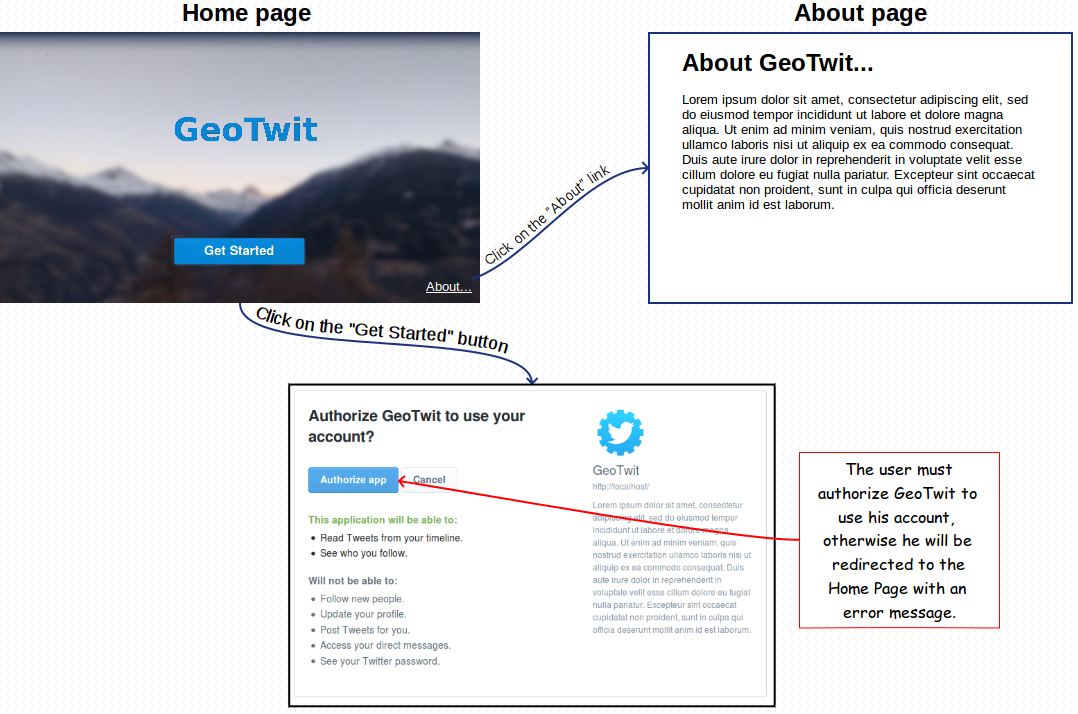
\includegraphics[width=\textwidth]{figures/mock-up-connection.png}}
\caption{mock-up - connection process}
\end{center}
\end{figure}
\newpage
\vspace*{\fill}
Once the connection is established, the user accesses the search page and can search for Tweets either in dynamic or static mode. First have a look at the \textbf{dynamic mode} (sometimes also called "streaming mode" in the application), which uses the Twitter's Streaming API.
\bigskip
\begin{figure}[H]
\begin{center}
\fbox{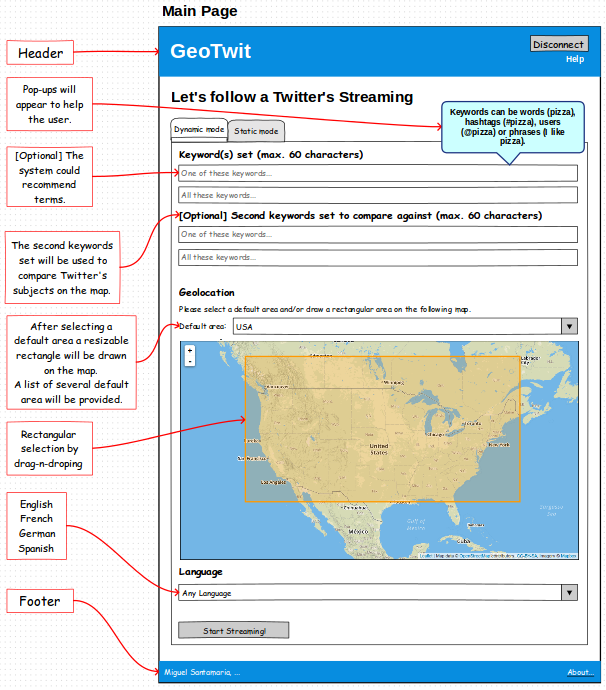
\includegraphics[width=\textwidth]{figures/mock-up-dynamic-mode-search.png}}
\caption{mock-up - main search page (dynamic mode)}
\end{center}
\end{figure}
\vspace*{\fill}
\newpage
\vspace*{\fill}
The user has to fill the fields, then click on the "Start Streaming!" button to begin the streaming process.
\bigskip
\begin{figure}[H]
\begin{center}
\fbox{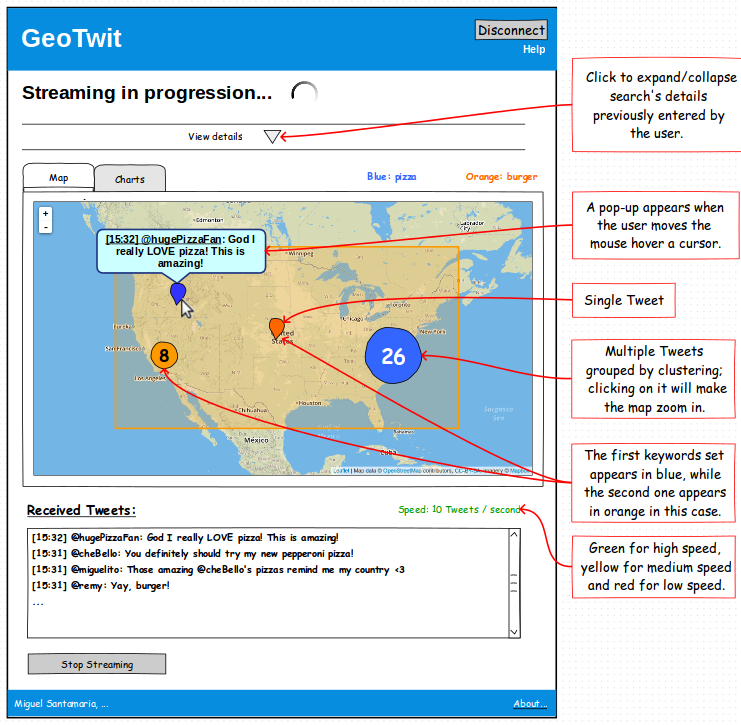
\includegraphics[width=\textwidth]{figures/mock-up-streaming-process.png}}
\caption{mock-up - streaming process}
\end{center}
\end{figure}
\vspace*{\fill}
\newpage
% Vertically center the text
\vspace*{\fill}
When watching the results, the user can also access the "Charts" tab, in which he can found interesting charts about the current streaming.
\bigskip
\begin{figure}[H]
\begin{center}
\fbox{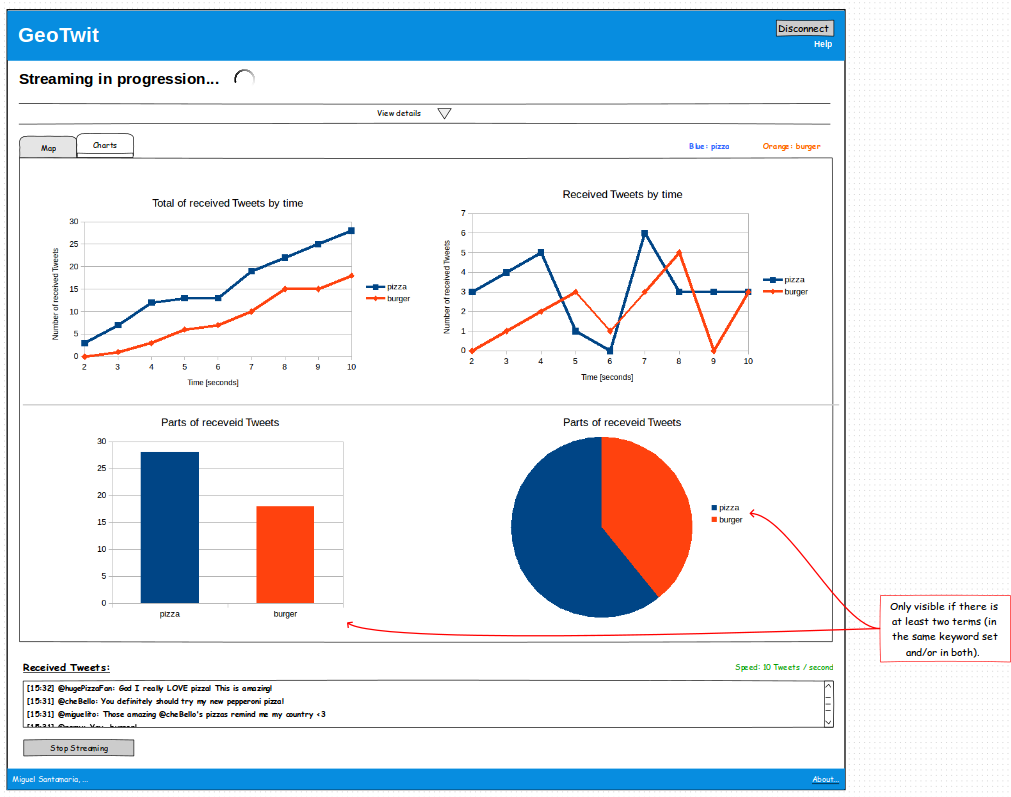
\includegraphics[width=\textwidth]{figures/mock-up-charts.png}}
\caption{mock-up - charts of a streaming process}
\end{center}
\end{figure}
\vspace*{\fill}
\newpage
\vspace*{\fill}
And now let's have a look at the \textbf{static mode}, which uses the Twitter's REST API.
\begin{figure}[H]
\begin{center}
\fbox{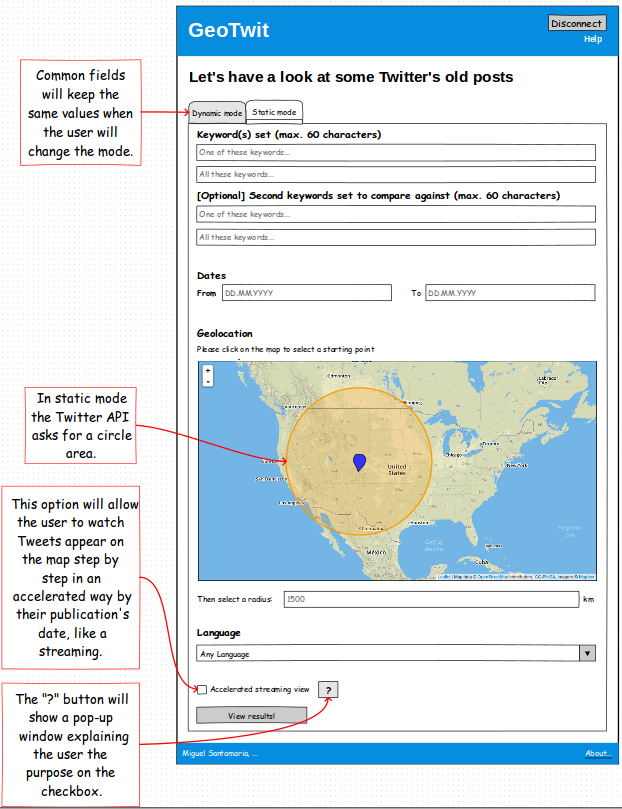
\includegraphics[width=0.9\textwidth]{figures/mock-up-static-mode-search.png}}
\caption{mock-up - main search page (static mode)}
\end{center}
\end{figure}
\vspace*{\fill}
\newpage
\vspace*{\fill}
Here again the user has to properly fill the fields and click on the "View results!" button in order to access the results.
\begin{figure}[H]
\begin{center}
\fbox{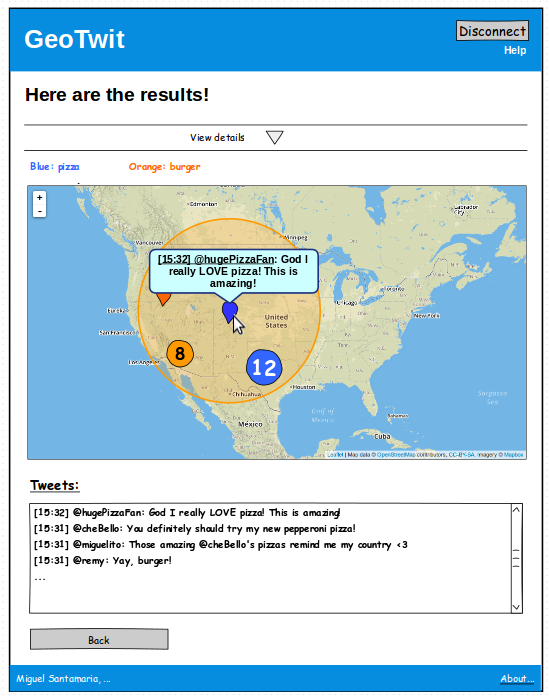
\includegraphics[width=0.8\textwidth]{figures/mock-up-static-results.png}}
\caption{mock-up - view of the results in the static mode}
\end{center}
\end{figure}
In the static mode, there is no charts.
\vspace*{\fill}
\newpage

\section{Anatomy of the Application}
\begin{wrapfigure}{l}{0.35\textwidth}
\vspace{-25pt}
\begin{center}
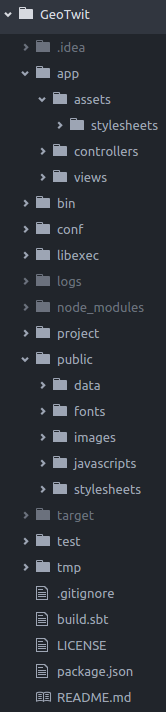
\includegraphics[width=0.26\textwidth]{figures/anatomy.png}
\caption{anatomy of GeoTwit}
\end{center}
\vspace{-100pt}
\end{wrapfigure}
Here is the anatomy\footnote{More information here: https://www.playframework.com/documentation/2.5.x/Anatomy} of the application:
\begin{itemize}
\item \textbf{app}: contains all components related to the server, like controllers, views and assets.
	\begin{itemize}
	\item \textbf{assets}: contains Less\footnote{http://lesscss.org/} files, which are converted to CSS files when the server compiles the code.
	\item \textbf{controllers}: contains all the application's controllers and actions, which act like standard API endpoints. It also contains actions compositions (see the "\nameref{actionsCompositions}" chapter below for more information).
	\item \textbf{views}: contains all views and sub-views of the application.
	\end{itemize}
\item \textbf{conf}: contains all the application's configurations, in particular the routes' configuration file.
\item \textbf{logs}: contains the application's logs file.
\item \textbf{node\_modules}: contains all the client's NPM\footnote{https://www.npmjs.com/} packages; you can find more information about them in the "\nameref{usedJavascriptLibraries}" chapter below.
\item \textbf{public}: contains files related to the build's properties of the project.
	\begin{itemize}
	\item \textbf{data}: contains Json and Shapefile data files, that respectively contain all the possible search's languages and the border's data of nearly all the territories of the world's countries.
	\item \textbf{javascript}: contains the Search page's JavaScript file as well as various JavaScript libraries (see the "\nameref{usedJavascriptLibraries}" chapter below for more details).
	\item \textbf{stylesheets}: contains the various JavaScript libraries' CSS files.
	\end{itemize}
\item \textbf{build.sbt}: this file is used to build the application and contains the application's description, library dependencies, resolvers and a filter used to automatically compile the Less code.
\end{itemize}
Other files and folders are not important and are in particular used by Activator and SBT to start and compile the application.
\newpage

\section{Implementation Details - Server Side}
\subsection{UML Diagram of the Server}
Here the UML diagram of the application's server, made with an old Bachelor project of the HEIG-VD, \emph{Slyum}\footnote{https://github.com/HEIG-GAPS/slyum}:
\begin{figure}[H]
\begin{center}
\fbox{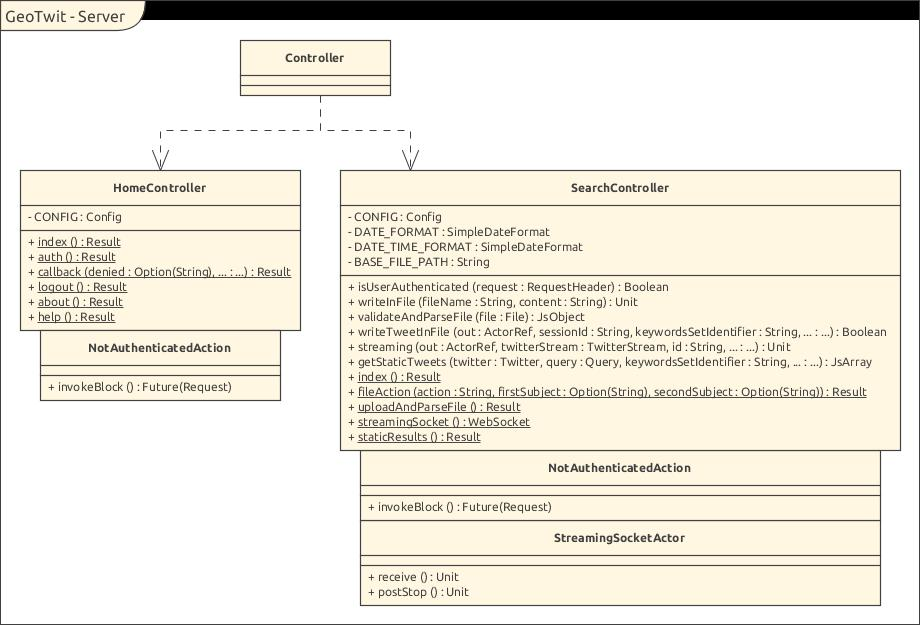
\includegraphics[width=0.8\textwidth]{figures/uml.jpg}}
\caption{UML diagram of the application's server, made with Slyum}
\end{center}
\end{figure}
The controllers' actions are underlined in this schema; the blocks attached at the bottom of the controllers are subclasses: "NotAuthenticatedAction" are actions compositions classes used to check if the user is correctly connected before accessing an action (see the "\nameref{actionsCompositions}" chapter below); "StreamingSocketActor" is the class that represents a WebSocket actor / thread (also see the "\nameref{webSockets}" chapter below).
Certain parameters of the "callback" method of the \textbf{HomeController} as well as the "writeTweetInFile", "streaming" and "getStaticTweets" methods of the \textbf{SearchController} were explicitly removed from the schema because of their numbers and thus because of the place they took. Here are the three methods' complete signatures: 
\begin{itemize}
\item \emph{callback(denied: Option[String], oauthToken: Option[String], oauthVerifier: Option[String]): Result}
\item \emph{writeTweetInFile(out: ActorRef, sessionId: String, keywordsSetIdentifier: String, internalId: Int, creationDate: String, longitude: Double, latitude: Double, user: String, content: String): Boolean}
\item \emph{streaming(out: ActorRef, twitterStream: TwitterStream, id: String, isAreaRectangle: Boolean, keywordsSetIdentifier: String, query: String, southwestCoordinates: Array[Double], northeastCoordinates: Array[Double], language: String): Unit}
\item \emph{getStaticTweets(twitter: Twitter, query: Query, keywordsSetIdentifier: String, maximumNumberOfRequests: Int): JsArray}
\end{itemize}
The \textbf{SearchController} entity does not contain all attributes, because it would have been too pompous to have them all; the missing ones are the constant variables that contain the backup file's string values (\textit{\textsc{metadata\_string}}, which contains "METATADA:", etc.).\\
As you can see, there is two controllers: \textbf{HomeController} and \textbf{SearchController}.\\\\
\textbf{HomeController} is related to all actions linked to the Home and miscellaneous pages, and the connection provess:
\begin{enumerate}
\item $\textbf{\underline{index}}\to$ displays the Home page and an error is the flash scope "error" is set (see the "\nameref{sessionsAndFlashScopes}" chapter).
\item $\textbf{\underline{auth}}\to$ occurs when the user clicked on the "Get Started" or "Connect" buttons of the Home page; redirects the user on the Twitter's connection page, giving it the URL of the callback function, which corresponds to the "callback" action below.
\item $\textbf{\underline{callback}}\to$ redirects the user either on the Search page if the connection was successful or on the Home page if there was an error or if the user denied the connection process. The status of the connection process depends on the three optional parameters: if "denied" is set, this means that the user denied the connection process and that the two following parameters are null. If "denied" is not set, this means that the two following parameters must have a value, respectively the token's string value (which will be used for the next requests to the APIs) and the "verifier" of the Twitter's OAuth process as a string (which will be asked by Twitter to verify the requests).\\
This action is called anyway by the Twitter's API when the user leaves the Twitter's connection page.
\item $\textbf{\underline{logout}}\to$ logs the user out and redirects him to the Home page.
\item $\textbf{\underline{about}}\to$ displays the About page; the user do not have to be authenticated to access this page.
\item $\textbf{\underline{help}}\to$ displays the Help page; the user do not have to be authenticated to access this page.
\end{enumerate}

\textbf{SearchController} is related to the Search page (search and display of the results); all parameters are explained directly in the code so they are not detailed again here; all actions necessitate the user to be connected:
\begin{enumerate}
\item $\textbf{isUserAuthenticated}\to$ checks if the user is correctly authenticated and returns a boolean value; this method is used by Ajax actions by the "AuthenticatedAction" actions composition.
\item $\textbf{writeInFile}\to$ writes the given string value in the given file's name, and it used to write the data in the file-to-export.
\item $\textbf{validateAndParseFile}\to$ Validates and parses the given file-to-import in order to export its data within the application; the file must be a well-formatted GeoTwit file (".gt" extension, containing metadata, tweets and results).    
\item $\textbf{writeTweetInFile}\to$ writes the Tweets whose information are given in parameters in the file to export.
\item $\textbf{streaming}\to$ starts a new Twitter's streaming process, according to the given parameters.
\item $\textbf{getStaticTweets}\to$ collects the Tweets associated to the given query with the given Twitter object, by not exceed the given limit of requests.
\item $\textbf{\underline{index}}\to$ displays the Search page, allowing the user to search Tweets with the Twitter's APIs.
\item $\textbf{\underline{fileAction}}\to$ gets the file containing the last streaming's results and either downloads or deletes it, depending on the given "action" parameter; returns a BadRequest result if the file or the given action do not exist.
\item $\textbf{\underline{uploadAndParseFile}}\to$ parses and validates the uploaded file to import.
\item $\textbf{\underline{streamingSocket}}\to$ this special action opens a WebSocket's connection (through the internal "StreamingSocketActor" class) between a new server's actor (thread) and the client when this one accesses this entity; this connection receives and sends Json values.
\item $\textbf{\underline{staticResults}}\to$ gets and returns the results of the static mode's search, when the user pressed the "View Results" of the "Static Mode" tab in the Search page.
\end{enumerate}
More information are given about these actions and methods in the following chapters.

\subsection{Behaviour of the Views}
All action's views inherit from one of these two interface templates: 
\begin{itemize}
	\item \emph{mainIndex.scala.html} if the current page is the home page. It contains only the header and footer partials and calls the page's content.
	 \item \emph{main.scala.html} for all other pages; in addition to contain the page's header and footer, it also contains a page content format, which allows the views to have the same page format (page's header, content, page's footer, etc.) in all pages.
\end{itemize}
As said above there is a header (\emph{header.scala.html}) and a footer (\emph{footer.scala.html}) partial templates, which are loaded in all templates. They respectively contain all HTML headers (page's title, CSS and libraries loading, etc.) and footers (closing tags).\\\\
The \emph{search.scala.html} search page's view is separated in three partial templates: \emph{searchContent.scala.html}, which contains the search fields of both dynamic and static modes, and \emph{searchStreamingResults.scala.html} and \emph{searchStaticResults.scala.html}, which respectively contain the components of the dynamic and static results' pages.

\subsection{Configuration}
Configuration files are located in the "/conf" folder. You can found the routes' configuration file in here, as well as the application and Twitter's configuration files.\\\\
The Twitter's file contains the consumer's key and secret used to make requests to the APIs. They are in a file apart in order to avoid security issues: the developer can indeed only push the application's configuration file (which contains non-confidential data) in the GitHub repository and keep the Twitter's file in local.
\newpage
In order to be able to read the configuration in the code, the developer has to inject a Configuration object in the controller in which he wants to use it:
\begin{figure}[H]
\vspace{-5pt}
\begin{center}
\fbox{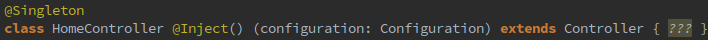
\includegraphics[width=\textwidth]{figures/configuration-injection.png}}
\vspace{-20pt}
\caption{injection of a Configuration object in a controller}
\end{center}
\end{figure}

\subsection{Routes}
\subsubsection{Play Router}
Routes\footnote{More information here: https://www.playframework.com/documentation/2.5.x/ScalaRouting} are set in the "/conf/routes" file, and are declared with three distinct parameters: the HTTP method (GET, POST, etc.), the URL of access ("/auth", etc.) and the controller and action in which the client will be redirected ("controller.HomeController.auth", etc.) and which can have parameters. They will be used by the server's routing process in order to determinate what to do with the given URL.\\\\
Note that there is also a route configured for the assets files (images, CSS, JavaScript, etc.), so the client can access all these files.
\bigskip

\subsubsection{JavaScript Routes}
In addition of the Play's main Scala routes and according to the documentation\footnote{https://www.playframework.com/documentation/2.5.x/ScalaJavascriptRouting}, the Play router is able to generate JavaScript code to handle routing from JavaScript running client side back to the application. The JavaScript router aids in refactoring the application; for example, when an URL or a parameter's name is changed, the JavaScript code will automatically get the new structure.
In GeoTwit, JavaScript routing is used in the Search page of the application. Specifically, JavaScript routes are declared in the "search.scala.html" view and are used in the "search.js" file:
\begin{itemize}
	\item \textbf{search.scala.html}: JavaScript routes are declared with a helper that generates the JavaScript code of a router named \emph{jsRoutes}. This router contains five routes: the route of the Logout page (in order to redirect the user from the JavaScript code if he is not connected anymore), the one of the "streamingSocket" of the SearchController (in order to initialize a web socket's connection with the server, see the "\nameref{webSockets}" chapter below), the "fileAction" action (in order to either delete of download the file-to-export from the JavaScript code), the "staticResults" action (in order to ask the server for the static mode's results), and finally a router for the assets files (in order to access images, fonts and other public assets).
	\begin{figure}[H]
	\vspace{-5pt}
	\begin{center}
	\fbox{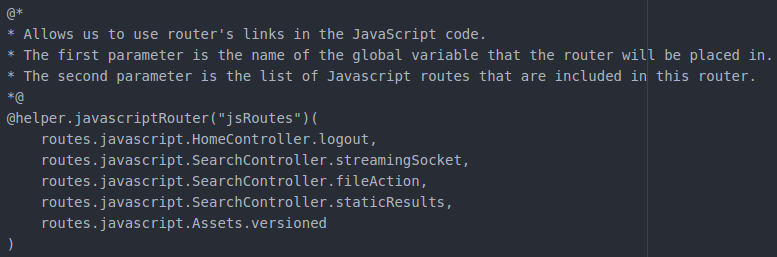
\includegraphics[width=0.64\textwidth]{figures/javascript-routes-declaration.png}}
	\vspace{-5pt}
	\caption{declaration of JavaScript routes in the Search page's view}
	\end{center}
	\end{figure}
	In order to make the helper work, the developer has to include the request's header as a parameter of the view: 
	\begin{figure}[H]
	\vspace{-5pt}
	\begin{center}
	\fbox{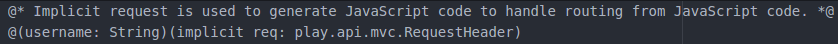
\includegraphics[width=0.86\textwidth]{figures/implicit-request-inclusion.png}}
	\vspace{-5pt}
	\caption{declaration of JavaScript routes in the Search page's view}
	\end{center}
	\end{figure}
	\vspace{-20pt}
	\item \textbf{search.js}: JavaScript routes are used with the \emph{jsRoutes.controllers.[CONTROLLER\_NAME]. [ACTION\_NAME]()} code. If one wants to access an asset entity (like an image or a font), it must replace the controller and action's names by the \emph{Assets.versioned('ASSET\_NAME')} code. It is then possible to get the URL of the current entity with the "url" method (which will for example generate the following link: "http://localhost:9000/logout") or also get a web socket's URL with the "webSocketURL" method (which could generate the following link: "ws://localhost:9000/streamingSocket").
	\begin{figure}[H]
	\vspace{-5pt}
	\begin{center}
	\fbox{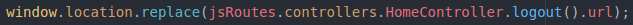
\includegraphics[width=0.86\textwidth]{figures/javascript-route-redirection.jpg}}
	\vspace{-5pt}
	\caption{example of redirection to the Logout page with a JavaScript route}
	\end{center}
	\end{figure}
\end{itemize}


\subsection{Sessions and Flash Scopes}
\label{sessionsAndFlashScopes}
In Play Framework, sessions do not really act like anyone might guess, because of the stateless status of the framework: according to the documentation\footnote{https://www.playframework.com/documentation/2.5.x/ScalaSessionFlash}, data are indeed not stored by the server, but are added to each subsequent HTTP request, using the cookie mechanism. This means that we can only store string values, and not objects. Since this limitation is very annoying, the developer has to use the cache mechanism to store objects (like the Twitter's signed object used to make requests in GeoTwit), by adding an unique ID related to the current user's session for each cached data (see the "\nameref{cache}" chapter below).\\\\
Each value stored in the session is identified by a string key and have a string value (like a "$String\to$ String" map). In order to add a value in the session, the developer has to use the "withSession" method right after the action's result (\emph{Ok}, \emph{Redirect}, etc.). Since sessions' data are added in each HTTP request, he has to get the current request's session and put it first in the new request's session in order to keep the older session's data.
\begin{figure}[H]
\vspace{-5pt}
\begin{center}
\fbox{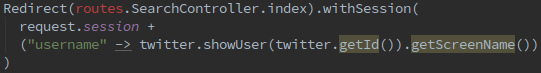
\includegraphics[width=0.86\textwidth]{figures/session-add-string-example.jpg}}
\vspace{-5pt}
\caption{example of addition of a string value in the session}
\end{center}
\end{figure}
\vspace{-10pt}

If one wants to set a new session, it just have to ignore the current request's session by removing the "request.session" call. In order to discards the whole session (during a disconnection for example), use the "withNewSession" method right after the action's result.\\\\
The session's time-out value is set in the "conf/application.conf" configuration file, specifically in the "play.http.session.maxAge" section. The value currently is 7 days.
\newpage
In GeoTwit, there can be two information contained in the session:
\begin{itemize}
	\item \textbf{id}: an unique ID used to identify the current user's session and especially the cache objects. This ID is indeed used to name and identify these cache objects (since the cache is not related to one user initially and is shared to everybody). This ID is generated with the Java's UUID generator and is set in the "auth" action of the \textbf{HomeController}.
	\item \textbf{username}: the username of the connected user, which is displayed in the header of the Search pages and is used to know if the user is connected or not (coupled with the cache - see the "\nameref{actionsCompositions}" chapter below). This value is set right after the Twitter's connection, in the "callback" action of the \textbf{HomeController}.
\end{itemize}

In addition of sessions, the framework also offers another tool: the flash scope. This mechanism works like sessions, with the difference that data are kept for only one request. It is used in GeoTwit to forward success/errors codes when an action redirect the user to the Home page.
\begin{figure}[H]
\vspace{-5pt}
\begin{center}
\fbox{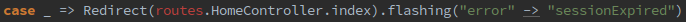
\includegraphics[width=\textwidth]{figures/flash-scope-use.jpg}}
\vspace{-20pt}
\caption{example of use-case of a flash scope in GeoTwit}
\end{center}
\end{figure}
\vspace{-10pt}

The index action of the \textbf{HomeController} gets the flash message and sends it to the view, which displays (or not) the right message, according to the status. If there is no error, the controller just sends a "success" message to the view.

\subsection{Cache}
\label{cache}
As said before, the cache\footnote{https://www.playframework.com/documentation/2.5.x/ScalaCache} is used to store objects that cannot be stored in sessions. Though, there is one main problem with this method: each time the server compiles a new code, the cache is cleared so the current connected users will be disconnected. When the application will be put in production environment, this problem will not occur that often.\\\\
In order to use the cache, add the "cache" library dependency in the \emph{build.sbt} file (normally already done by default), then inject a \emph{CacheApi} object in the controller in which you want to use the cache functionalities:
\begin{figure}[H]
\vspace{-5pt}
\begin{center}
\fbox{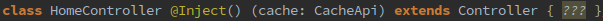
\includegraphics[width=\textwidth]{figures/cacheapi-injection.jpg}}
\vspace{-20pt}
\caption{injection of a CacheApi object in a controller}
\end{center}
\end{figure}
\vspace{-10pt}

It is then possible to use this "cache" object to read and write the cache.\\
When an object is added in the cache, the developer can set a time value, which will determinate the period of validity of this object; once the limit is reached, the object will be removed from the cache.
\begin{figure}[H]
\vspace{-5pt}
\begin{center}
\fbox{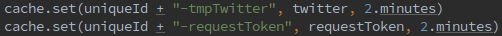
\includegraphics[width=0.8\textwidth]{figures/cache-timer.jpg}}
\vspace{-5pt}
\caption{example of addition of objects in the cache, for a 2 minutes' period}
\end{center}
\end{figure}
\vspace{-10pt}

\newpage
In order to read a cache object, this one must be converted in the right type (a RequestToken object in the example below):
\begin{figure}[H]
\vspace{-5pt}
\begin{center}
\fbox{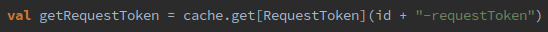
\includegraphics[width=0.8\textwidth]{figures/cache-reading.jpg}}
\vspace{-5pt}
\caption{example of reading of a cache object}
\end{center}
\end{figure}
\vspace{-10pt}

The developer has to think about testing the collected object's existence, in order to ensure it is still available.\\\\
Here are the different objects that can be stored in the cache in GeoTwit ("[id]" represents the unique ID generated for the current session, in order to differentiate the cache objects stored on the server side between each connected client):
\begin{itemize}
	\item \textbf{[id]-tmpTwitter} (2 minutes' validity)\\
	Contains the \textbf{Twitter} object used to get the \underline{request} token and the Twitter's authentication URL. This object is stored in the "auth" action of the \textbf{HomeController} and is collected in the "callback" action right after the Twitter's connection. It has to be stored, because it has already been signed with the \underline{request} token, and still has to be signed with the \underline{access} token in the callback, in order to be able to make requests to the APIs. This object is thus reused to build the final \textbf{Twitter} object, and since it is not possible to build a new object for security issues, it has to be kept.\\
	If this object times out before the user reached the callback, he will be redirected to the Home page with an explicit error.
	\item \textbf{[id]-requestToken} (2 minutes' validity)\\
	Also stored in the "auth" action and used in the "callback" action, this object contains the current user's request token, which will be used to generate the access token. If this object times out before the user reached the callback, he will be redirected to the Home page with an explicit error.
	\item \textbf{[id]-twitter} (currently have a 7 days' validity, which is the same value as the session's time-out and is stored in the application's configuration file)\\
	Contains the \textbf{Twitter} final and signed object, which will be used to make requests to the Twitter's APIs in the \textbf{SearchController}. It is set in the "callback" action of the \textbf{HomeController}, right after the two cached object above has been removed from the cache. If this object expired for one reason or another, the user will be considered as disconnected and thus will be redirected to the Home page.
\end{itemize}

\subsection{Twitter4J}
Twitter4J is used in the \textbf{HomeController} and is automatically loaded by SBT with the \emph{build.sbt} file. As said before, this file indeed contains the Twitter4J's library dependency:
\begin{lstlisting}
	org.twitter4j" % "twitter4j-core" % "4.0.4
\end{lstlisting}
The first string is the library's location, the second one is the library's name and the last one is the library's version. In order to use the streaming API, the file also has to contain the Twitter4J's stream library: 
\begin{lstlisting}
	org.twitter4j" % "twitter4j-stream" % "4.0.4
\end{lstlisting}

\subsection{Connection Process}
In order to properly implement the connection process, the code is based on the \emph{yusuke}'s implementation example of a connection process to Twitter with the Twitter4J library in Java\footnote{Available on GitHub here: https://github.com/yusuke/sign-in-with-twitter} as well as a \emph{Qiita}'s tutorial\footnote{http://qiita.com/omiend/items/90163d29b465fb7ab8f0}.\\\\
When the user clicks on the "Get Started" button located in the Home page, the following steps are operated:
\begin{enumerate}
	\item The click action calls the "auth" method of the \textbf{HomeController}.
	\item This action uses the Twitter4J library to make an authentication's request, in order to get the OAuth token and the authentication URL that points to the Twitter's authorization page. When making the request, the application also gives the API a callback URL (\emph{/callback} => action "callback" of the \textbf{HomeController}), which will be called at the end of the authentication. This action also stores the temporary Twitter's and request token's objects in the cache for 2 minutes, in order to properly use them in the callback action.
	\item Redirection of the user to the Twitter's authorization page.
	\begin{figure}[H]
	\vspace{-5pt}
	\begin{center}
	\fbox{
\includegraphics[width=0.85\textwidth]{figures/twitter-authorization-page-in-geotwit.jpg}}
	\vspace{-5pt}
	\caption{Twitter's authorization page in the GeoTwit application}
	\end{center}
	\end{figure}
	\vspace{-20pt}
	\item Whatever the user does, he will be redirected on the callback action: 
	\begin{enumerate}
		\item If the user successfully authorized the application, the callback receives the OAuth token and verifier from Twitter. It will then get and memorize the OAuth \underline{access} token (according to the temporary Twitter and \underline{request} token's objects received from the "auth" action, as well as the received verifier from Twitter), add the new Twitter's object in the cache for 7 days (same time as the session's time-out) in order to use it in the \textbf{SearchController} to make requests to the APIs, and then finally redirect the user to the "search" action, passing the username in the session (in order to display it on the pages' header).
		\item If something went wrong, the user is redirected on the Home page with an error.
	\end{enumerate}
\end{enumerate}
\newpage

\subsection{Actions Compositions}
\label{actionsCompositions}
Actions compositions\footnote{More information here: https://www.playframework.com/documentation/2.5.x/ScalaActionsComposition} can be interpreted like generic action functionalities, allowing the developer to execute generic code in several actions without writing it again. In summary, this code is executed before the execution of the action itself; compositions thus act like filters (which contain code executed before any action when a request is made to the Play server), but for specific actions, and can be chained by forwarding the HTTP request through a pipeline-like process.
\begin{figure}[H]
\vspace{-5pt}
\begin{center}
\fbox{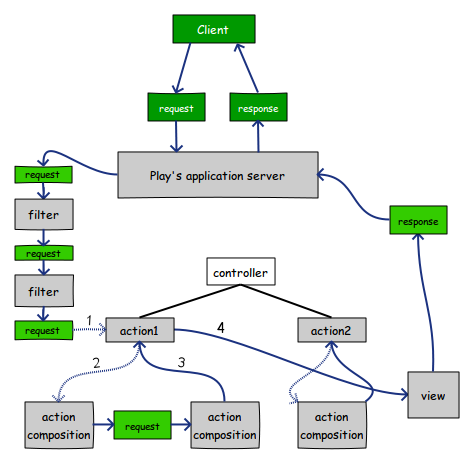
\includegraphics[width=0.9\textwidth]{figures/filters-actions-compositions.png}}
\vspace{-5pt}
\caption{pipeline-like schema of filters and actions compositions, made with Evolus Pencil}
\end{center}
\end{figure}
\vspace{-10pt}
In the above schema, the client first makes a request to the Play's application server, which sends it to the first filter. This filter executes its code and can perhaps modify the request's content; once done, he forwards the updated request to the next filter, and so on. When the request is finally forwarded to the right controller's action (through the routing process), this one calls the actions compositions related to itself, which alternately execute their code and can also update the request. Once the last action composition finished its process, the request is finally forwarded to the action, whose body's code is executed and in which a result (for example the call of the view with the \emph{Ok} keyword) will be provided.
\newpage
In GeoTwit, actions compositions are used to check if the user is connected or not before accessing pages: for all the \textbf{HomeController}'s actions (except the "logout", "about" and "help" ones), the user is redirected to the Search page if he is already connected; on the opposite, if the user is not connected and tries to access a \textbf{SearchController}'s action, he will be redirected to the Home page with an error message. In order to determinate if an user is disconnected or not, the actions compositions check if the "username" value of the session is set and if a \emph{[id]-twitter} object exists in the cache for the current session (where "[id]" represents the unique ID of the current session). If one of these two values does not exist (or if the unique ID is not set), the user is considered as disconnected.\\\\
These actions compositions are objects extending the \textbf{\emph{ActionBuilder}} trait (the \textbf{\emph{NotAuthenticatedAction}} object in the \textbf{HomeController}, and the \textbf{\emph{AuthenticatedAction}} object in the \textbf{SearchController}), and implementing a "invokeBlock" method, which is called for every action built by the \textbf{\emph{ActionBuilder}}.
\begin{figure}[H]
\vspace{-5pt}
\begin{center}
\fbox{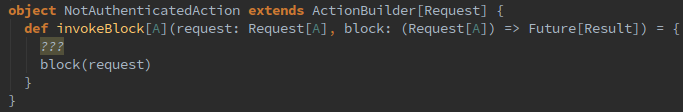
\includegraphics[width=\textwidth]{figures/actions-composition-example.jpg}}
\vspace{-20pt}
\caption{an example of an actions composition}
\end{center}
\end{figure}
\vspace{-10pt}

The "request" parameter of the "invokeBlock" method corresponds to the current HTTP request's object. The "block" parameter is a function used to wrap the request, by giving a future result to the HTTP request and thus by allowing the request to be chained until the last actor (the action itself).\\\\
Actions are then defined with these objects, in order to execute the "invokeBlock" method's code before the action itself.
\begin{figure}[H]
\vspace{-5pt}
\begin{center}
\fbox{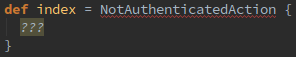
\includegraphics[width=0.45\textwidth]{figures/action-using-actions-composition.jpg}}
\vspace{-6pt}
\caption{an action using an actions composition}
\end{center}
\end{figure}
\vspace{-10pt}

\subsection{Web Sockets}
\label{webSockets}
According to the documentation\footnote{https://www.playframework.com/documentation/2.5.x/ScalaWebSockets}, web sockets are sockets that can be used from a web browser based on a protocol that allows a two way full duplex communication. Both the client and the server can send and receive messages at any time, as long as there is an active web socket connection between them. In summary, one can use this technology to forward real-time messages from a client to a server and vice-versa; in GeoTwit, web sockets are used to forward data during the streaming process.
\newpage
In order to make the web socket's communication work, the application thus must have a web socket's client ans server entities. In GeoTwit, the client is a JavaScript part located in the "search.js" file (modern HTML5 compliant web browsers natively support web sockets via JavaScript), and the server is located in the \textbf{SearchController}. Play provides two different mechanisms for handling web sockets: by using Akka Streams and by using iteratees. Since this second method is deprecated, it will not be explained below and Akka is the one which is used in the application.\\\\
Since it would be annoying to split the server and the client parts' explanations, they are both explained here.
\begin{figure}[H]
\vspace{-5pt}
\begin{center}
\fbox{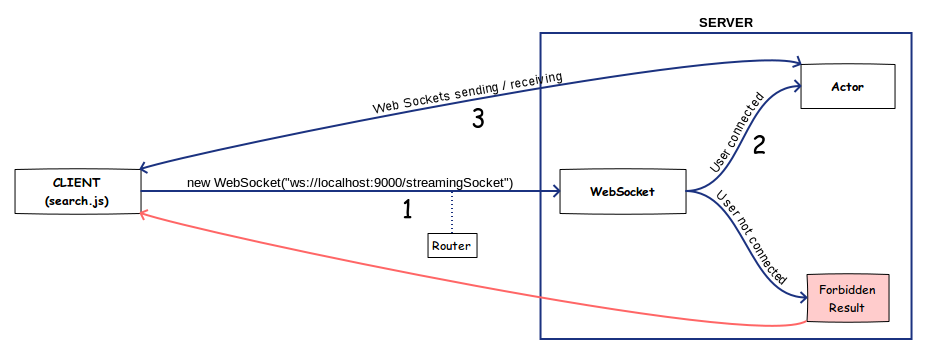
\includegraphics[width=\textwidth]{figures/web-sockets.png}}
\vspace{-20pt}
\caption{diagram of the web sockets' process is Play Framework, made with Evolus Pencil}
\end{center}
\end{figure}
\vspace{-15pt}

In order to be able to send web sockets between a client and the server, a connection firstly has to be initialized. In GeoTwit, the following process is executed:
\begin{enumerate}
	\item The client has to open a new web socket connection to the server, with the web socket protocol (\emph{ws://[URL\_OF\_SERVER]}). A route is declared in the server's router in order to redirect the client's request to the right entity (which is not exactly an action in this case, but a \emph{WebSocket} object).
	\begin{figure}[H]
	\vspace{-5pt}
	\begin{center}
	\fbox{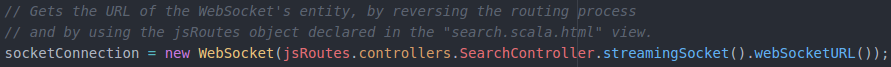
\includegraphics[width=0.86\textwidth]{figures/web-socket-connection-openning.jpg}}
	\vspace{-5pt}
	\caption{opening of a new web socket connection from the client to the server}
	\end{center}
	\end{figure}
	\vspace{-20pt}
	
	\item The \emph{WebSocket} object of the server acted like an action until now, but no more from here. Once it received the client's connection request, it indeed checks that the current user is still authenticated (for security reasons) and if so, it creates a new \emph{Actor} object through an \emph{ActorFlow} object that allows the developer to access a "out" \emph{ActorRef} object that will itself be used to send messages to the client. This \emph{Actor} object acts like a Java Thread, which means it will keep a persistent connection with the client until the expressed closing of this connection (web browser's closing, reload of the current page, expressed web socket message indicating the server that the connection has to end, etc.), and which also means that the server can proceed other processes at the same time. In summary, the \emph{WebSocket} object acts like a threads manager while the \emph{Actor} objects act like threads; there can indeed be several current \emph{Actor} instances running at the same time, but only one connection's \emph{WebSocket} object, which ends as soon as the \emph{Actor} is created.\\
	In GeoTwit, the \emph{WebSocket} object also gives the \emph{Actor} the session's unique ID, so it will be able to access the current user's cache object. Note that the \emph{WebSocket} object (and thus the \emph{Actor} one) is configured to only accept and send Json data (in Play: \emph{JsObject/JsValue} objects\footnote{https://www.playframework.com/documentation/2.5.x/ScalaJson}), so it will be easier to identify and deal with web sockets' types. If the user is not connected anymore when the server receives a connection request, this one sends back a Forbidden result that will make the client disconnect the user.
	\item Once the \emph{Actor} threaded object is created, it immediately sends a "successfulInit" message to the client, in order to notify it that the connection was successfully opened. As said before, only Json objects can be sent and received in GeoTwit.\\\\
	In order to send sockets to the client, the \emph{Actor} object has to use the given \emph{ActorRef} ("out") object:
	\begin{figure}[H]
	\vspace{-5pt}
	\begin{center}
	\fbox{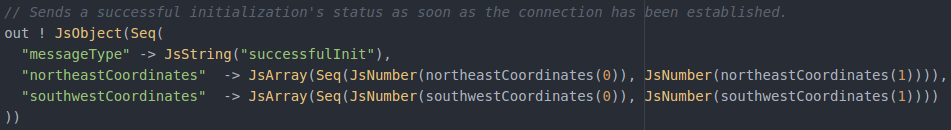
\includegraphics[width=0.86\textwidth]{figures/web-socket-sending-server-to-client.jpg}}
	\vspace{-5pt}
	\caption{example of a web socket's sending from the server to the client}
	\end{center}
	\end{figure}
	\vspace{-20pt}
	
	When a message is sent from the client, the \emph{Actor} receives it with the "receive" method. This method gets the received Json message's type and process actions depending on it.\\
	Finally, the "postStop" method is triggered when the web socket's connection ended, and is used to properly close the current running streaming. In order to manually ends the \emph{Actor} threaded object, the developer has to send a \emph{PoisonPill} object to the \emph{ActorRef} ("out") object with the following command:
	\begin{lstlisting}
		out ! PoisonPill
	\end{lstlisting}
	
	\item On the client side, everything is managed with the \emph{socketConnection} object, initialized when the client first sent a connection request to the server. This object contains several methods, among which the "onmessage" one that is triggered when the client receives a message from the socket. Like in the server side, when a message is received, the client first gets the received Json message's type and process actions depending on it.
\end{enumerate}
\bigskip
Here are the messages that can be sent \underline{from the server to the client} in GeoTwit (the first Json object's attribute is the message type, sometimes followed by various parameters):
\begin{itemize}
	\item \textbf{\{"successfulInit"\}}: sent when the client's connection request has been successfully received by the server; when the client receives it, it shows the results page, draws the selected area (rectangle or complex polygon) on the results map and sends back a "readyToStream" message to the server.
	\item \textbf{\{"newTweet", \textit{keywordsSet}, \textit{internalId}, \textit{creationDate}, \textit{longitude}, \textit{latitude}, \textit{user}, \textit{content}, \textit{nbReceivedTweets}\}}: sent when a new Tweet has been received through the Twitter's streaming process; the client adds the Tweet to the map, displays it in the results panel, and sends a confirmation to the server, indicating that the Tweet belongs to the country's territories (if so and only if the user selected the country in the drop-down menu ; see the client's "readyToStream" and "tweetLocationConfirmation" web sockets for more information).\\The "keywordsSet" parameter indicates the keywords set's identifier (either "first" or "second") to which the Tweet belongs (so the client can display Tweets with different colors). "internalId" contains the internal ID of the Tweet, used to identify Tweets in the file-to-export. "creationDate" contains the creation date of the Tweet, "longitude" and "latitude" are the Tweet's geographic coordinates, "user" contains the name of the user who posted the Tweet and "content" contains the Tweet's content. Finally, "nbReceivedTweets" contains the current number of received Tweets (with or without geolocation tags), used by the graphs.
	\item \textbf{\{"errorFile"\}}: sent when an error occurred during the creation/writing of the file-to-export by the server. An alert is displayed in order to inform the user, but the streaming process continues.
	\item \textbf{\{"stopStreaming", \textit{reason}\}}: sent when the server stopped the streaming process (mainly in case of exception); indicates the client that he can itself indicate the user that the streaming ended. The "reason" is an optional parameter that indicates the reason of this stop, which can be:
	\begin{itemize}
		\item \emph{sessionExpired}: when the server cannot access the Twiter's cached object anymore, which means that the current user's session has expired; the client redirects the user to the Logout page in order to properly disconnect him. This error can only happen at the beginning of the streaming process, when the server tries to initialize the streaming connection with the Twitter's API; once done, the cached object is not used anymore and the streaming can continue (in order to avoid annoying disconnections during the process).
	\item \emph{tooManyStreamingProcesses}: when the user ran too many (more that two) copies of the same application that are authenticated with the same account.
	\item \emph{queryTooLong}: when the user typed too many characters in one of the keywords sets (more than 60 in one \underline{OR} phrase - see the "\nameref{buildingTwitterQueryString}" chapter of the client side below); the search page is reloaded in order to make a new search.
	\item \emph{exception}: when a non-handled exception occurred; displays an alert window.
	\end{itemize}
\end{itemize}
\bigskip

Here are now the messages than can be sent \underline{from the client to the server}: 
\begin{itemize}
	\item \textbf{\{"readyToStream", \textit{isAreaRectangle}, \textit{firstKeywords}, \textit{secondKeywords}, \textit{coordinates}, \textit{language}\}}: sent as soon as the client received a "successfulInit" message from the server; when the server receives this message, he starts the Twitter's streaming process(es) with the given user's input parameters. "isAreaRectangle" indicates whether the user manually drew a rectangle on the map (\emph{true}) or selected a country in the drop-down menu (\emph{false}); if \emph{false}, this value indicates that the server must wait for the client to send a confirmation that indicates that the received Tweet is in the complex polygon area that represents the country's territories (since the client only gave the bounding box to the server, in order to avoid to overload the connection - see the figure below), in order to only write Tweets belonging to the area in the file to export; if the value is \emph{true}, the server will automatically write Tweets in the file, without asking the client a confirmation. "secondKeywords" can be empty, since it is an optional input. "language" contains a BCP 47 language identifier\footnote{https://en.wikipedia.org/wiki/IETF\_language\_tag} ("en", "fr", etc.) that corresponds to the value of the language the user selected to filter Tweets (if empty, the system will simply not filter Tweets by language).	The "coordinates" parameter is an array that contains each coordinates of a rectangle's corners; this rectangle can either be the rectangle the user manually drew, or the rectangle bounding all the selected country's territories (since a country can have many of them) in the user selected a country in the drop-down menu. Here is an example of a bounding rectangle for the France territories (aka France and Corsica):
	\begin{figure}[H]
	\vspace{-5pt}
	\begin{center}
	\fbox{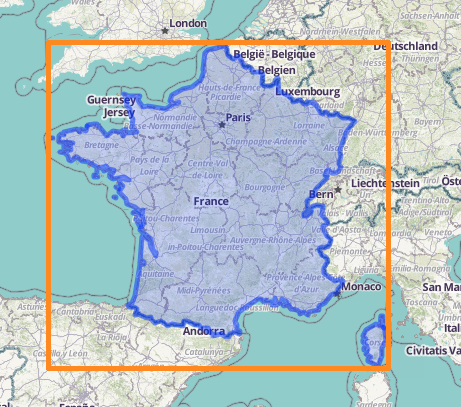
\includegraphics[width=0.85\textwidth]{figures/france-bounding-rectangle-example.jpg}}
	\vspace{-5pt}
	\caption{example of a rectangle bounding the France's territories}
	\end{center}
	\end{figure}
	\vspace{-20pt}
	
	Since it is not possible to send huge amounts of data like the coordinates of all the country's borders through the web sockets system (and even if it was possible, it is really not optimized), the client only sends this bounding rectangle. Once received, the server will search for Tweets contained within this rectangle, and will send them to the client, which will finally check that the Tweet belongs to one of the country's territories (see the client side's "\nameref{receptionOfTweetsFromTheServer}" chapter below for more information).
	
	\item \textbf{\{"currentResults", \textit{elapsedTime}, \textit{gtrt}, \textit{grt}, \textit{gprt}, \textit{atrt}, \textit{art}, \textit{agvw}\}}: sent each second by the client; gives the server the current results (the elapsed time, and the data related to each of the 6 charts: $\textbf{gtrt}\to$ Total of received geolocated Tweets; $\textbf{grt}\to$ Reception of geolocated Tweets; $\textbf{gprt}\to$ Parts of the received geolocated Tweets; $\textbf{atrt}\to$ Total of all (with and without geolocation) received Tweets; $\textbf{art}\to$ Reception of all Tweets; $\textbf{agvw}\to$ Tweets with geolocation tags vs. Tweets without; more information about charts in the "\nameref{charts}" chapter of the client side's section). The server internally saves and overwrites these results, in order to write them at the end of the backup file once the streaming process ended.
	\newpage
	\item \textbf{\{"tweetLocationConfirmation", \textit{keywordsSet}, \textit{internalId}, \textit{creationDate}, \textit{longitude}, \textit{latitude}, \textit{user}, \textit{content}\}}: sent by the client in order to confirm that the received Tweet (received through the "newTweet" web socket) belongs to the selected country's territories, in order for the server to write it in the file to export. This socket is only sent if the user selected a country in the drop-down menu; indeed, only the bounding box is sent to the server at the beginning of the streaming process, in order to avoid overloading it (see the "readyToStream" web socket). If the Tweet does not belong to the territories, the client simply ignore it. The "keywordsSet" parameters indicates which subject the Tweet-to-confirm belongs to (either "first" or "second"), "internalId" is used to internally differentiate the Tweets to write and results from an internal server's counter, and "creationDate" is the Tweet's creation date, as a \emph{YYYY-MM-DD'T'hh:mm:ss} format. Other parameters are the basic Tweet's parameters.
	\item \textbf{\{"stopStreaming"\}}: sent when the user clicked on the "Stop Streaming" button; indicates the server that he can kill the current \emph{Actor} and stop the current Twitter's streaming process.
\end{itemize}
\newpage

Here is a summary of the communication that occurs between the server and the client:
\begin{figure}[H]
\vspace{-5pt}
\begin{center}
\fbox{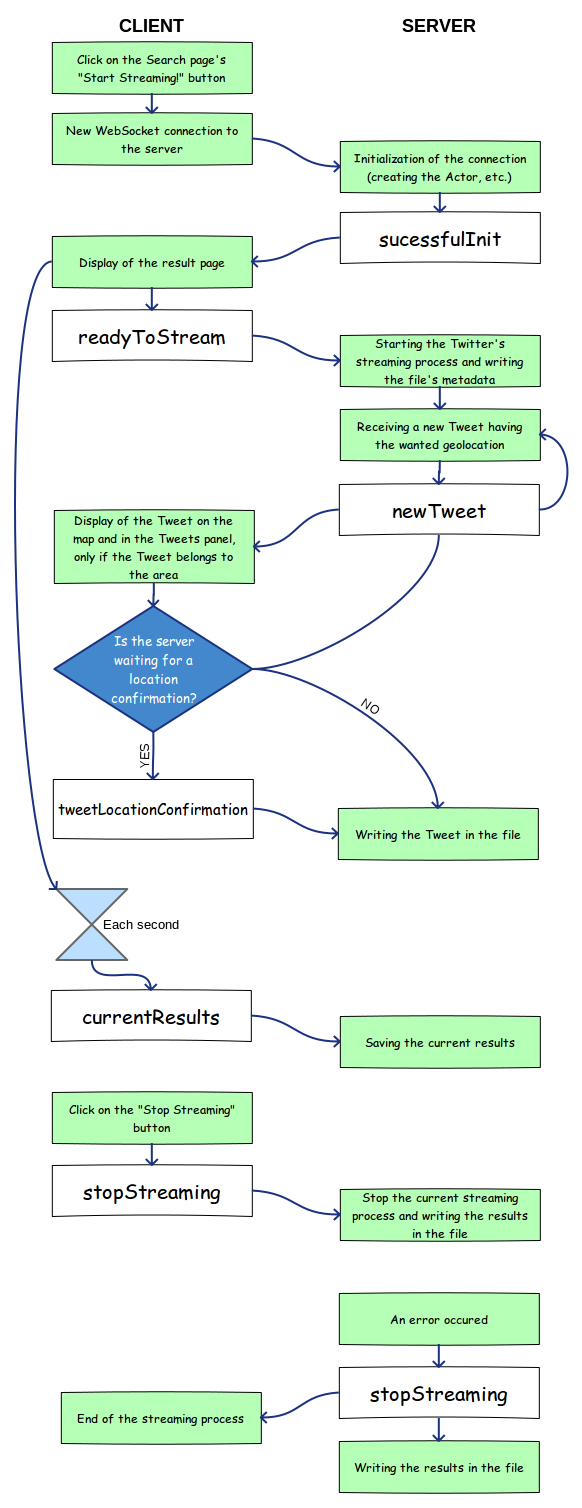
\includegraphics[width=0.53\textwidth]{figures/web-sockets-in-geotwit.png}}
\vspace{-5pt}
\caption{web sockets' operation diagram in GeoTwit, made with Evolus Pencil}
\end{center}
\end{figure}

\subsection{Streaming Processes}
Once the client sent all the data related to the streaming process(es) through the "readyToStream" web socket, the current web socket's \emph{Actor} of the server validates the user's parameters and checks that the user is still connected and if so, it starts the first streaming process through the Twitter's API with the Twitter4J library. If the user filled the second keywords set/subject, the \emph{Actor} starts a second streaming process. As a reminder, the Twitter's API only authorizes two simultaneous streaming per user, so it is not possible to add new keywords sets for now. The streaming process is located in the "streaming" method of the \textbf{SearchController}, and initializes a listener subscribed to a server of the Twitter's Streaming API with the both the right query's parameters and a \emph{TwitterStream} object initialized from the cached Twitter object. Once a Tweet is received, it will trigger the "onStatus" method of the listener object, which will check if the Tweet have a geolocation tag and if so, if it is geolocated in the wanted rectangle. If so, the \emph{Actor} will send a "newTweet" web socket to the client.\\\\
If a user deletes a Tweet previously poster, the information will be received in the "onDeletionNotice" method of the listener object; though, deletions are ignored in GeoTwit, since a Tweet still deserve to appear in the results, even if it was deleted. If an exception occurs during the streaming process, the "onException" method of the listener object will be triggered. This one tries to convert the \emph{Exception} object into a \emph{TwitterException} object, in order to get the exception's status code and thus to properly inform the client about what happened through the "stopStreaming" web socket.\\\\
Everything is well commented in the code, so it would be useless to explain everything right here.

\subsection{Generation and Exportation of the Files during the Streaming Mode}
\label{generationOfStreamingFile}
At the end of a streaming process, the user is asked to either export or not the backup file of the analysed subject(s) generated during the process. Both the client and the server take action during this process, but everything is explained here, in order to avoid useless mixes.\\\\
First thing first, here is the format of the generated text file:
\begin{figure}[H]
\vspace{-5pt}
\begin{center}
\fbox{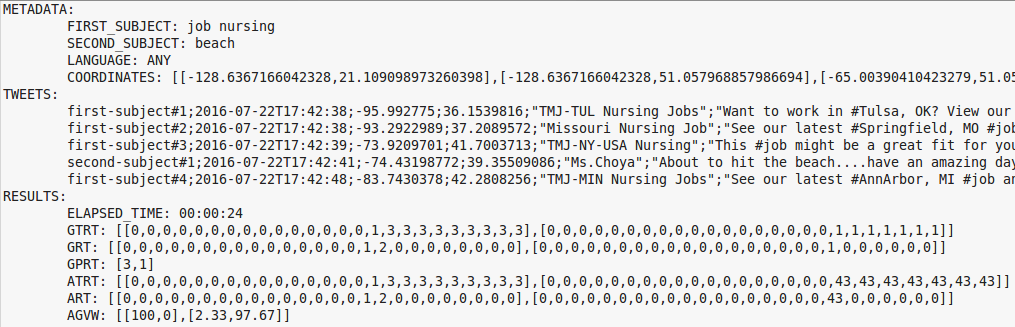
\includegraphics[width=\textwidth]{figures/generated-file-format.jpg}}
\vspace{-5pt}
\caption{format of the generated text file that contains streaming process(es) data}
\end{center}
\end{figure}

\textit{Spaces and tabulations were added in this example in order to make the file more readable; in real files, there is such things as spaces or tabulations, in order to gain space.}\\\\
And here are the explanations:
\begin{itemize}
	\item \textbf{METATADA}: his section contains the metadata of the current streaming process and is located at the beginning of the file. The metadata contain: 
	\begin{itemize}
		\item the \textbf{first subject's search-string};
		\item the \textbf{second subject's search-string}, only if the user set a second keywords set; if not, this line does not exist;
		\item the \textbf{language} used to filter the Tweets ("ANY" if the user did not select a specific language);
		\item the \textbf{coordinates} used to filter the Tweets, as a string-representation of an array of arrays of double (see the illustration above to have an example).
	\end{itemize}
	
	\item \textbf{TWEETS}: this section contains the data of all received geolocated Tweets, and is located after the metadata. There is strictly one Tweet per line, and each Tweet contains the following information, separated by semicolons:
	\begin{itemize}
		\item the \textbf{identifier} of the current Tweet, which is formatted  as the following: \\"\emph{[SUBJECT\_IDENTIFIER]-subject-\#[TWEET\_ID]}", where \emph{[SUBJECT\_IDENTI-FIER]} corresponds to the string identifier of the subject with which the Tweet has been found (either "first" or "second"), and where \emph{[TWEET\_ID]} corresponds to the local counter value of Tweets received for the current subject until now (in order to identify Tweets of a same subject between them);
		\item the \textbf{date and time} that represent the creation of the current Tweet, following a \emph{YYYY-MM-DD'T'hh:mm:ss} format, where '\emph{T}' is a simple character used to separate the date from the time (and which is used by the Scala parser in order to convert this string into a date);
		\item the \textbf{longitude} of the Tweet;
		\item the \textbf{longitude} of the Tweet;
		\item the \textbf{name of the user} who posted the Tweet, bounded by quotation marks (in case the user's name contains a semicolon);
		\item the \textbf{text content} of the Tweet, also bounded by quotation marks for the same reason; if a Tweet's content contains line breaks, they are automatically removed.
	\end{itemize}
	
	\item \textbf{RESULTS}: this section contains the results of the streaming process, and is located at the end of the file, after the tweets. The results contains:
	\begin{itemize}
		\item the \textbf{time} the process lasted, formatted as a \emph{hh:mm:ss} format;
		\item the \textbf{graphs' data} (one line per graph: $\textbf{GTRT}\to$ Total of received geolocated Tweets; $\textbf{GRT}\to$ Reception of geolocated Tweets; $\textbf{GPRT}\to$ Parts of the received geolocated Tweets; $\textbf{ATRT}\to$ Total of all (with and without geolocation) received Tweets; $\textbf{ART}\to$ Reception of all Tweets; $\textbf{AGVW}\to$ Tweets with geolocation tags vs. Tweets without). All graphs have a two-dimensions array of two arrays of numbers, except the GPRT one, which only have a simple array of numbers. If a chart does not exist (if there is only one subject the GPRT one will not exist, for example) or is empty, an empty array is written (for example: "\underline{[[],[]]}", or "\underline{[]}" for the GPRT).
	\end{itemize}
	Since all the collected Tweets are public, there is no confidentiality issues about the storage of these data in an external file.
\end{itemize}

During the process, the file is firstly created in the "writeInFile" method of the \textbf{SearchController}, if it is not already existing on the server side. This method writes the given string value in the file whose name corresponds to the given string. For the streaming processes, the files are located in the "/tmp" file and are named as the following: \emph{streaming-[ID].gt}, where \emph{[ID]} corresponds to the unique ID of the current session of the connected user. Every connected user thus has a file having a unique name for his current session. This also means that there can only be one file per session, which allows the server to not be overloaded by files. \emph{gt} is the self-assigned official extension of GeoTwit files, but is just a text file in reality. Note that the file is deleted once it has been downloaded or rejected, but the process is explained later in this chapter.\\\\
The first time the "writeInFile" method is called (and thus the file is created) occurs in the "receive" method of the \emph{StreamingSocketActor} class of the \textbf{SearchController}, when the "readyToStream" web socket type is received and when the user's inputs have been validated by the server. This first call allows the server to write the metadata of the current streaming process at the beginning of the file.\\\\
Then, this method is called each time the server receives a new Tweet from the Twitter's server, either in the "onStatus" method of the listener located in the "streaming" method of the \textbf{SearchController}, or in the "receive" method of the \emph{StreamingSocketActor} class, when the actor received a "tweetLocationConfirmation" web socket type (depending if the user respectively manually drew a rectangle on the map or selected a country in the countries' list - more information in the "\nameref{webSockets}" chapter above). This call writes the received/confirmed Tweet in the file.\\\\
Each second, the client sends the current elapsed time and the charts results to the server (with the "currentResults" web socket), which overwrites them each time. As soon as the streaming process is stopped (either because an exception was thrown or because the user clicked the stop button), the server writes the last received results at the end of the file (still with the same "writeInFile" method). Simultaneously, the client asks the user if he wants to export the generated file, in the "stopStreaming(...)" function of the \emph{search.js} file. If the user says \emph{yes}, he will be able to download the file; if he says \emph{no}, the file will directly be removed from the server, in order to keep it clean at every time. Note that the user is well warned about the results of his decision.
\begin{figure}[H]
\vspace{-5pt}
\begin{center}
\fbox{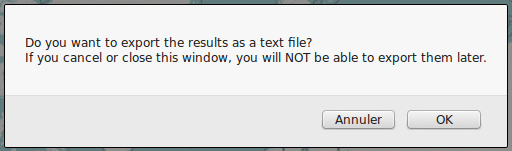
\includegraphics[width=0.7\textwidth]{figures/export-data-pop-up.jpg}}
\vspace{-5pt}
\caption{pop-up asking the user if he wants to export the data as a text file (french buttons are due to the browser's default language)}
\end{center}
\end{figure}

In order to easily download the file and to get a feedback about the download process (either a success or a failure), the \emph{johnculviner}'s "jquery.fileDownload" Jquery's download library\footnote{https://github.com/johnculviner/jquery.fileDownload} was used. It allows the developer to use an Ajax-like file-download experience, which is normally not (easily) possible by using the web.\\
The developer just needs to call the library, giving it the URL of the action from which the user can download the file. In GeoTwit, this action is the "fileAction" action of the \textbf{SearchController}, which is used either to download or delete the current user's file (you can find more information in the following paragraphs). Here is a sample of code, which is used to download the file:
\begin{figure}[H]
\vspace{-5pt}
\begin{center}
\fbox{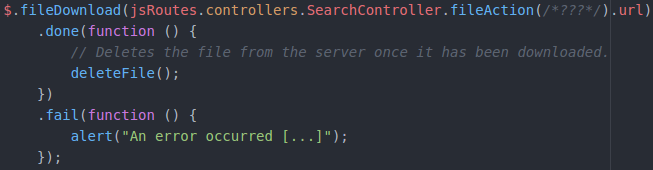
\includegraphics[width=0.7\textwidth]{figures/jquery-filedownload-sample.jpg}}
\vspace{-5pt}
\caption{sample of code used to download the generated file}
\end{center}
\end{figure}

Once the download finished, the file is immediately removed from the server, thanks to the "deleteFile" function of the \emph{search.js} file. If an error occurred, an alert message containing the URL of the download page is displayed to the user, so he can manually download it. Note that the next time the user will press the "Start Streaming!" button, the file will automatically be removed (in order to avoid keeping useless files on the server side).\\\\
The "deleteFile()" function only sends an Ajax request to the "fileAction" action of the \textbf{SearchController}, in order to delete the file. It does not wait for a response from the server.\\\\
Regarding the "fileAction" action of the \textbf{SearchController}, this one either downloads or deletes the current user's file, according to its first's string parameter (which can either be "download" or "delete"). This action also needs the string(s) that represents the keywords set(s), in order to properly name the file to download. It first gets the file on which the action will be operation, and checks if this file exists. If not, a \emph{BadRequest} response is returned; if yes, the server performs the wanted action. If the file must be deleted, the server simply execute the "delete" method of the file object; if the file must be downloaded, the server has to serve it to the client. In order to accomplish this task, the action must render a file instead of an HTTP result\footnote{More information here: https://www.playframework.com/documentation/2.5.x/ScalaStream}:
\begin{figure}[H]
\vspace{-5pt}
\begin{center}
\fbox{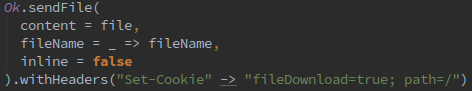
\includegraphics[width=0.6\textwidth]{figures/rendering-file-in-action.jpg}}
\vspace{-5pt}
\caption{rendering of a file at the end of an action}
\end{center}
\end{figure}

The content contains the \emph{java.io.File} object to send; the file name contains the name of the file that the user will see in the download pop-up, and is formatted as the following: \\\emph{[SUBJECT\_1][\_[SUBJECT\_2]]\_STREAMING\_[DATETIME].gt}, where \emph{[SUBJECT\_1]} and \emph{[SUBJECT\_2]} (optional) represent the keywords sets' strings, and where \emph{[DATETIME]} represents the current date and time, following a \emph{YYYY-MM-DD'T'hh\_mm\_ss} format. The "inline" parameter indicates if the file must be served as an inline file (which means that he is directly displayed in the web browser instead of being downloaded through a pop-up).
\newpage
The "Set-Cookie" HTTP header added at the end of the \emph{Result} object is used by the "jquery.fileDownload" library in order to receive a confirmation when the file was successfully downloaded (an thus to remove it from the server).\\\\
You can finally find an example of generated file in the \emph{/tmp/EXAMPLE.gt} file.

\subsection{Importation of a Generated File}
GeoTwit also allows the user to import a previously generated file, in order to watch the results again (in a static way; the streaming does not resume). Here again, both the client and server sides are explained, in order to avoid mixes.\\\\
The user has the possibility to import a generated file by clicking a button located at the beginning of the Dynamic Mode tab's content. In summary, he has to click the button in order send the file to the "uploadAndParseFile" action of the \textbf{SearchController}, which will validate and parse the file, then send back the parsed data to the client as a Json format. You can find more details about this process in the paragraphs below.
\bigskip

\subsubsection{Client Side}
The upload process starts as soon as the user chose a file to upload. Firstly, in order to be able to send the file to the action with an Ajax request (for getting Json data back from the server at the end of the process) and to be able to display a progress-bar about the upload, the basic plugin of the \emph{blueimp}'s "jQuery-File-Upload" library\footnote{https://github.com/blueimp/jQuery-File-Upload}-\footnote{https://github.com/blueimp/jQuery-File-Upload/wiki/Basic-plugin for the basic plugin} is used.
\begin{figure}[H]
\vspace{-5pt}
\begin{center}
\fbox{
\includegraphics[width=0.9\textwidth]{figures/jquery-file-upload-progress-bar.jpg}}
\vspace{-5pt}
\caption{progress-bar managed by the jQuery-File-Upload library during an upload process}
\end{center}
\end{figure}

In order to initialize the automatic Ajax upload, the "fileupload" method is called on the "file" HTML input. The given parameters indicate that the client expects the server to answer with Json data and also provide the refresh function of the progress-bar.
\begin{figure}[H]
\vspace{-5pt}
\begin{center}
\fbox{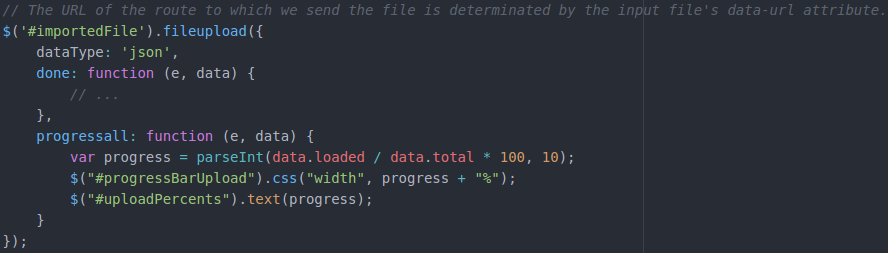
\includegraphics[width=0.95\textwidth]{figures/ajax-upload-process-initialization.jpg}}
\vspace{-5pt}
\caption{initialization of the automatic Ajax upload process on the "file" input}
\end{center}
\end{figure}

As mentioned in the code's comment, the URL of the route to which the client sends the file is determined by the HTML input file's "data-url" attribute, which contains the route of the "uploadAndParseFile" action.\\\\
The "progressall" function episodically calculates the current progression value of the progress-bar by the current loaded data (this number being received from the server), then refreshes the HTML components.\\\\
The "done" function is called when the upload process is complete: it displays an error if the Json data received from the server contain one, or otherwise calls the "loadFileResultsComponents(...)" function of the \emph{search.js} file, which loads the components (map, charts, HTML components) as well as the received data (display of the metadata, the Tweets and the results).
\bigskip

\subsubsection{Server Side}
On the server side, the "uploadAndParseFile" action first validate the file, which must exist and be a text file, and which cannot be empty. If a validation error occurs, the following Json object is returned:
\begin{itemize}
	\item \textbf{error}: \emph{true};
	\item \textbf{reason}: the reason key of the error, which is either "fileEmpty", "wrongFormat" or "missingFile".
\end{itemize}

If the file is valid, the action call the "validateAndParseFile(...)" method of the same controller, which validates the content of the file. This method returns a Json object containing either an error if there was one or the parsed data of the file if everything was valid: 
\begin{itemize}
	\item The file's content must first have the three "METADATA", "TWEETS" and "RESULTS" sections.
	\item The "\textbf{METADATA}" section must have at least the "FIRST\_SUBJECT" (\emph{String}), "LANGUAGE" (\emph{String}) and "COORDINATES" (array of arrays of \emph{Double}) values; the "SECOND\_SUBJECT" (\emph{String}) value is optional. The order of the values does not matter, as long as all of them (except the optional one) are present in this section.
	\item The "\textbf{TWEETS}" section can be empty (if there was no received Tweet during the analysis) and is directly followed by the "RESULTS" section in this case; if it contains Tweets, these have to be properly formatted (see the contained data in the "\nameref{generationOfStreamingFile}" chapter above): the date must be as the \emph{YYYY-MM-DD'T'hh:mm:ss} format, the longitude and latitude must be \emph{Double} types, and the user's name and Tweet's content must be bounded by quotation marks. There must be strictly one Tweet per line.
	\item The "\textbf{RESULTS}" section must contain the "ELAPSED\_TIME" (\emph{String}) value, and the data linked to the charts ("GTRT", "GRT", "ATRT", "ART", "AGVW" (arrays of two arrays of \emph{Double}, which can be empty => "\underline{[[],[]]}"), and GPRT (simple array of \emph{Double}, which can also be empty => "\underline{[]}")). The order does not matter here, as long as every of these values is contained in this section.
	\item There must not be useless spaces, tabulations or line breaks.
\end{itemize}

While parsing the file for validating it, the algorithm also simultaneously collects all the data in order to gain time; if a validation error occurs, these data are dropped. The algorithm is separated in three parts: 
\begin{itemize}
	\item Validation and collection of the "METADATA" section, and retrieval of the other section's start lines.
	\item Validation and collection of the tweets if the metadata were valid and if the file contains the two other sections.
	\item Validation and collection of the results if the two other parts were valid, then return of the Json results.
\end{itemize}

In order to validate and collect the values, the algorithm uses regular expressions with parentheses (in order to group data and get them as variables) and match cases to validate them. For example, if the algorithm wants to get the language value of the metadata, it will use the following regular expression, which will match a line beginning with "LANGUAGE:" and followed with a value containing at least one character:
\begin{figure}[H]
\vspace{-5pt}
\begin{center}
\fbox{
\includegraphics[width=0.5\textwidth]{figures/language-regex.jpg}}
\vspace{-5pt}
\caption{Regex used to match the language string in the imported file}
\end{center}
\end{figure}

The parentheses contained within the Regex (regular expression) are used to group the value in order to get it as a variable. The algorithm then tries to match the parsed file's lines with this regular expression, by collecting the group as a "l" variable.
\begin{figure}[H]
\vspace{-5pt}
\begin{center}
\fbox{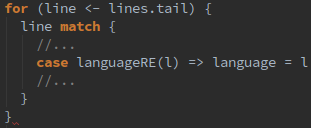
\includegraphics[width=0.5\textwidth]{figures/language-regex-matching.jpg}}
\vspace{-5pt}
\caption{matching of the regex used for the language}
\end{center}
\end{figure}

The validation of the other metadata and results applies the same principle. Tweets validation is a little more complicated: the Regex validates and collects 6 different variables separated by ';'.
\begin{figure}[H]
\vspace{-5pt}
\begin{center}
\fbox{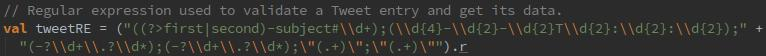
\includegraphics[width=\textwidth]{figures/tweet-regex.jpg}}
\vspace{-20pt}
\caption{Regex used to validate and get data of Tweets}
\end{center}
\end{figure}
\newpage

These variables must be in the following order and must be formatted as followed:
\begin{itemize}
	\item The Tweet's identifier, which must start either by "first" or "second" (the "?>" characters indicates Scala that we do not want to group the character contained in bounded parentheses as a variable), followed by "-subject\#", then by a number. For example: \underline{first-subject\#2}.
	\item The date, which must contains a string formatted as the following: \emph{XXXX-XX-XXTXX:XX:XX}, where 'X' is a digit and where 'T' is the \emph{'T'} character. For example: \underline{2016-07-22T15:30:14}.
	\item The longitude, which must be a double. For example: \underline{-87.9997769}.
	\item The latitude, which also must be a double. For example: \underline{47.8106521}.
	\item The user's name, which must contain at least one character and must be bounded by quotation marks (note that only the bounded content will be taken in the variable). Quotes are used to avoid bugs with a string that would contain a colon. For example: \underline{"Speedway Jobs"}.
	\item The content, which must follow the same rules as the user's name. For example: \underline{"Hello everybody!"}.
\end{itemize}

Once every value of the file is valid and collected, the method sends back a Json object, containing the following attributes:
\begin{itemize}
	\item \textbf{error}: \emph{false} (indicates that there was no error);
	\item \textbf{firstSubject}, \textbf{secondSubject} (can be an empty string), \textbf{language}, \textbf{coordinates};
	\item \textbf{tweets} => an array containing each Tweet's values: \textbf{subjectIdentifier} (either "first" or "second"), \textbf{dateAndTime}, \textbf{longitude}, \textbf{latitude}, \textbf{user} and \textbf{content};
	\item \textbf{results} => an object containing the results: \textbf{elapsedTime}, \textbf{gtrt}, \textbf{grt}, \textbf{gprt}, \textbf{atrt}, \textbf{art} and \textbf{agvw}.
\end{itemize}

If there was an error, the method sends back a Json object containing:
\begin{itemize}
	\item \textbf{error}: \emph{true};
	\item \textbf{reason}: the reason key of the error, which is "fileNotValid".
\end{itemize}

This object is forwarded to the client through the "uploadAndParseFile" action. If everything was valid, the client displays data on the screen.
\newpage

\subsection{Retrieving of Static Tweets}
\subsubsection{Issues due to Limitations}
Before explaining the concerned algorithms, more details have to be given about the work of the Twitter's REST API when a lot of data are available for the current user's request. Indeed, the Twitter's server cannot send the whole amount of data at one time from a certain number of Tweets, because of the problems that this action can cause (mainly slowness). In order to avoid these kinds of problems, Twitter sends the results by "pages", each page containing a certain amount (up to 100 - configurable with Twitter4J) of Tweets. If there is still too many results, the API also limits the number of pages, which complicates the process: indeed, the developer has to get the lowest ID of the received Tweets set, in order to make a new request that collects a new Tweets set from this ID. Here is an example with a maximum of \underline{three} Tweets per page, and a maximum of \underline{two} pages per results' set:
\begin{figure}[H]
\vspace{-5pt}
\begin{center}
\fbox{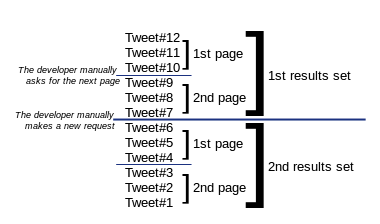
\includegraphics[width=0.8\textwidth]{figures/rest-api-limitations.png}}
\vspace{-5pt}
\caption{example of the limitations problem of the Twitter's REST API}
\end{center}
\end{figure}

In this example, the first request collects the Tweets from \#12 to \#7 (from the highest to the lowest IDs, because Twitter logically firstly sends the most recent Tweets), by generating two pages. The developer has to manually ask for the next page each time he collected all the Tweets of a page, and has to execute a new sub-request with the new page. Once the first request does not have pages anymore, the developer has to get the lowest ID of the retrieved Tweets (here: \#7) if order to make a new request to collect the Tweets from \#6, and so on.\\\\
This system raises a huge issue: like it was said before in the analysis part of this document, Twitter indeed limits the number of requests that a user can make in a 15 minutes' period. Since every page's sub-request is considered as a request, and since the user may have to do various requests to get all results, the limit can quickly be reached. For this reason, the number of results if limited in GeoTwit.\\\\
If this case occurs and the obtained results are limited, the user has to be more specific about his subject(s) and about the range of date. Twitter's REST API unfortunately only supports dates and is incompatible with times, so there is no way to be more specific than days.

\subsubsection{Algorithms}
When the user clicks on the search button of the static mode's page, the client makes an Ajax request to the server in order to retrieve the list of static Tweets (see the "\nameref{retrievalOfTweets}" chapter in the client's static part below). The server uses the Twitter's REST API to collect Tweets in the "staticResults" action of the \textbf{SearchController}; it first gets and validates the sent parameters, then creates the queries.
\begin{figure}[H]
\vspace{-5pt}
\begin{center}
\fbox{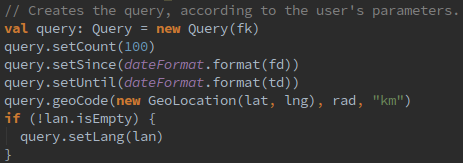
\includegraphics[width=0.7\textwidth]{figures/rest-api-query-creation.jpg}}
\vspace{-5pt}
\caption{creation of a query for asking the Twitter's REST API with Twitter4J}
\end{center}
\end{figure}

The "setCount" method is used to indicate the maximum number of Tweets per page (which can be up to 100 maximum). "setSince" and "setUntil" methods take a \emph{YYYY-MM-DD} date as a string value and are used to filter the Tweets respectively by their start and end dates.\\\\
The action then calls the "getStaticTweets(...)" method for each subject, which gets the Tweets related to the given parameters and builds a Json's array object with them. Specifically, this method applies the algorithm seen above about pages and results' sets in order to avoid limitations as much as possible. Firstly, the "maximumNumberOfRequests" parameters indicates the algorithm the maximum number of requests it can do before risking to reach the Twitter limit. After a few tests, it turns out that the maximum number of requests is close to 175 per account for a laps of 15 minutes (this value may be greater, but it seems to be the minimum value). The following example was generated by putting "println" after each request in the code:
\begin{figure}[H]
\vspace{-5pt}
\begin{center}
\fbox{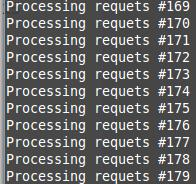
\includegraphics[width=0.4\textwidth]{figures/number-static-requests-before-error.jpg}}
\vspace{-5pt}
\caption{example of the number of requests executed before getting an error in a period of 15 minutes}
\end{center}
\end{figure}
\newpage

In order to keep a margin of error, this number is truncated to \textbf{170} in GeoTwit (approximately 17'000 Tweets), which means that if the user entered two different subjects, each search must at at most make \textbf{85} requests (approximately 8'500 Tweets per subject). This calculation is managed by the "staticResults" action: the maximum number is contained in the constant variable "MAXIMUM\_NUMBER\_OF\_REQUESTS"; when the action calls the "getStaticTweets(...)" method, it indicates the number of requests it can do by the number of subjects the user selected and by this constant value.\\\\
Due to these limitations and issues, the static mode is thus less developed than the streaming mode in GeoTwit. Also for the same reasons, \textbf{\underline{the "Accelerated Streaming View" tools that}} \textbf{\underline{was planned in the specifications was aborted}}; as a compromise, the file importation was developed in the dynamic mode.

\section{Implementation Details - Client Side}
\subsection{Both Streaming and Static Modes}
\subsubsection{Structure of the client's JavaScript file}
Since all the JavaScript code is contained in the \emph{/public/javascripts/search.js} file, there cannot be a decent UML schema. For this reason, here is the list of functions contained in this file (remember that JavaScript is a non-typed language), order by their order of appearance:
\begin{itemize}
	\item \emph{secondsToHhMmSs(seconds)}
	\item \emph{cloneObject(obj)}\cite{elliotbonneville2011}
	\item \emph{erasePolygons(map)}
	\item \emph{drawPolygons(map, coordinates, readFileMode)}
	\item \emph{invertCoordinates(coordinates)}
	\item \emph{isPointInSelectedArea(latitude, longitude, polygonsCoordinates)}\cite{RandolphFranklin2016}
	\item \emph{loadCountriesList()}
	\item \emph{loadLanguagesList()}
	\item \emph{loadSearchMap(mapId, hasRectangle, hasCircle)}
	\item \emph{loadStaticMap()}
	\item \emph{loadResultsMap(mode)}
	\item \emph{loadStreamingResultsCharts(hasSecondStream, refresh)}
	\item \emph{calculateAndDisplaySpeedValues()}
	\item \emph{loadStreamingResultsComponents()}
	\item \emph{loadFileResultsComponents(data)}
	\item \emph{loadStaticResultsComponents()}
	\item \emph{selectCountryOnMap(countryName, map)}
	\item \emph{initWebSocket()}
	\item \emph{stopStreaming(sendSocket, displayExportPopup)}
	\item \emph{deleteFile()}
	\item \emph{addTweetOnPage(mode, subjectNumber, latitude, longitude, date, user, content)}
	\item \emph{getStaticTweets()}
	\item \emph{validateDynamicFields()}
	\item \emph{validateStaticFields()}
	\item \emph{getAndFormatKeywords(keywordsSetNumber, mode)}
	\item \emph{\$(document).ready(function()}: occurs when the page successfully loaded all DOM elements.
\end{itemize}

Most of these functions are precisely explained in the following chapters.
\bigskip

\subsubsection{Used JavaScript Libraries}
\label{usedJavascriptLibraries}
Several JavaScript external libraries are used in GeoTwit, in order to avoid reinventing the wheel when there are already great existing libraries doing the work we want to do. About half of them are NPM\footnote{https://www.npmjs.com/} packages located in the \emph{/node\_modules} directory, which the other half are external JavaScript libraries found on the web and being located in the \emph{/public/javascripts} directory.
\begin{enumerate}
	\item \textbf{NPM packages}:
	\begin{itemize}
		\item \textbf{Chart.js}\footnote{http://www.chartjs.org/}: allows the developer to draw simple and responsive HTML5 charts.
		\item \textbf{Leaflet}\footnote{http://leafletjs.com/}: allows the developer to build interactive maps coupled with OpenStreetMap.
		\item \textbf{Leaflet.markercluster}\footnote{https://github.com/Leaflet/Leaflet.markercluster}: this plug-in for Leaflet is used to automatically group markers by clusters on the maps.
		\item \textbf{Leaflet.draw}\footnote{https://github.com/Leaflet/Leaflet.draw}: a vector drawing and editing plug-in for Leaflet, used to draw rectangles and circles on the maps (by being coupled with the next library).
		\item \textbf{Leaflet.draw.drag}\footnote{https://github.com/w8r/Leaflet.draw.drag}: this library is used coupled with the \emph{Leaflet.draw} one, in order to allow the user to draw and drag polygons (rectangles and circles) on the maps with a special toolbar.
		\item \textbf{Moment.js}\footnote{http://momentjs.com/}: allows the developer to parse, validate, manipulate, and display dates in JavaScript.
	\end{itemize}
	\newpage
	
	Since NPM packages must normally be used with a Node.js server, the NPM package "browserify"\footnote{http://browserify.org/} is used. As a reminder, this package allows the developer to use NPM's packages within a simple JavaScript's client application.  As soon as the \emph{/public/javascripts/search.js} file is updated, the developer has to type the following command in a console to generate the \emph{/public/javascripts/search-bundle.js} file.
	\begin{lstlisting}
		browserify search.js -o search-bundle.js
	\end{lstlisting}
	This \emph{search-bundle.js} file contains a working version of the \emph{search.js} file, with all the code of the NPM's packages included in it. This file is thus the one that is read by the web browser
	
	\item \textbf{External JavaScript libraries}:
	\begin{itemize}
		\item \textbf{jQuery}\footnote{https://jquery.com/}: provides easier way to manipulate DOM elements than simple JavaScript code.
		\item \textbf{Bootstrap}\footnote{http://getbootstrap.com/}: provides HTML components, CSS classes and JavaScript code to easily develop responsive interfaces.
		\item \textbf{shapefile-js}\footnote{https://github.com/calvinmetcalf/shapefile-js}: the \emph{calvinmetcalf}'s library provides a tool to read Shapefile-formatted\footnote{https://en.wikipedia.org/wiki/Shapefile} files and parse them in Json.
		\item \textbf{pickadate.js}\footnote{http://amsul.ca/pickadate.js/}: provides JavaScript date and time pickers.
		\item \textbf{jquery.fileDownload}\footnote{https://github.com/johnculviner/jquery.fileDownload}:  the \emph{johnculviner}'s library provides an easy way to download file with Ajax requests.
		\item \textbf{jQuery-File-Upload}\footnote{https://github.com/blueimp/jQuery-File-Upload}: the \emph{blueimp}'s library is used to easily upload files with Ajax and to show a progress-bar.
	\end{itemize}
\end{enumerate}

Several of these libraries was already encountered before in this document; the rest of them will be properly explained in the following chapters.
\bigskip

\subsubsection{Dates Format}
Since a lot of dates are used in GeoTwit (in the static mode's search page, and in the results pages of both modes) and since they have to be regularly formatted, validated and converted to string objects, the "Moment.js" library is used to simplify these processes. This well-known library indeed allows the developer to easily work with dates of both \emph{Date} and \emph{String} types.
\newpage

\subsubsection{Building of the Twitter's Query String}
\label{buildingTwitterQueryString}
In order to filter Tweets with the Twitter API, the developer has to give a query string. It is possible to add \underline{AND} and \underline{OR} filter's operator by respectively separating the words with spaces (" ") and commas (",") for the streaming mode or with the " OR " and " AND " strings for the static mode, since parentheses are not supported by the API. Note that the \underline{AND} keyword takes priority over the \underline{OR} one, since comma-separated terms are considered as phrases by the API; here are some examples with the streaming mode (the method is the same for the static mode):
\begin{itemize}
	\item $job\to$ interpreted as "job"
	\item $job engineer\to$ job \underline{AND} engineer
	\item $job,engineer\to$ job \underline{OR} engineer
	\item $job engineer,nursing\to$ (job \underline{AND} engineer) \underline{OR} nursing
	\item $job,engineer nursing\to$ job \underline{OR} (engineer \underline{AND} nursing)
	\item $job,engineer nursing,potato\to$ job \underline{OR} (engineer \underline{AND} nursing) \underline{OR} potato
\end{itemize}

Once the user filled the keywords sets (with spaces between words) and pressed the search button, the "getAndFormatKeywords(...)" function is called. There cases are possible from there:
\begin{enumerate}
	\item The user only filled the AND part ("All these keywords...") $\to$ there is nothing to do here since the words are already separated by spaces.
	\item The user only filled the OR part ("One of these keywords...") $\to$ the algorithm replaces the spaces with commas.
	\item The user filled the AND and the OR parts $\to$ since the \underline{AND} takes priority over the \underline{OR} and since we want to search Tweets that contain all the AND words and one of more of the OR words (for example: "(dog \underline{AND} cat) \underline{AND} (eat \underline{OR} drink)", the algorithm has to manually build the string, by taking each of the OR words and by adding them one by one at the end of the AND words, separating all the possibilities with commas. For example, if the user entered "\textbf{dog cat}" in the AND field and "\textbf{eat drink}" in the OR field, the resulted query will be "\textbf{dog cat eat,dog cat drink}", which is interpreted as "(dog \underline{AND} cat \underline{AND} eat) \underline{OR} (dog \underline{AND} cat \underline{AND} drink)".
\end{enumerate}

According to the documentation, the text of the Tweet and some entity fields are considered for matches. Specifically, the text attribute of the Tweet, the "expanded\_url" and "display\_url" values for links and media, the text for hashtags, and the "screen\_name" value for user mentions are checked for matches. Each phrase of the query (terms between commas, like "\textbf{dog cat eat}" and "\textbf{dog cat drink}") must contains up to 60 characters maximum, otherwise the API will generate an error.
In all cases, the function also locally saves a human-comprehensive query (with "\underline{AND}" and "\underline{OR}" keywords, and parentheses), in order to display it in the results page. These queries are generated by parsing the query sent to the server.
\newpage

\subsubsection{Selection of the Language of the Tweets}
In GeoTwit, the user can choose a language with a drop-down menu, in order to filter the received Tweets by their language.
\begin{figure}[H]
\vspace{-5pt}
\begin{center}
\fbox{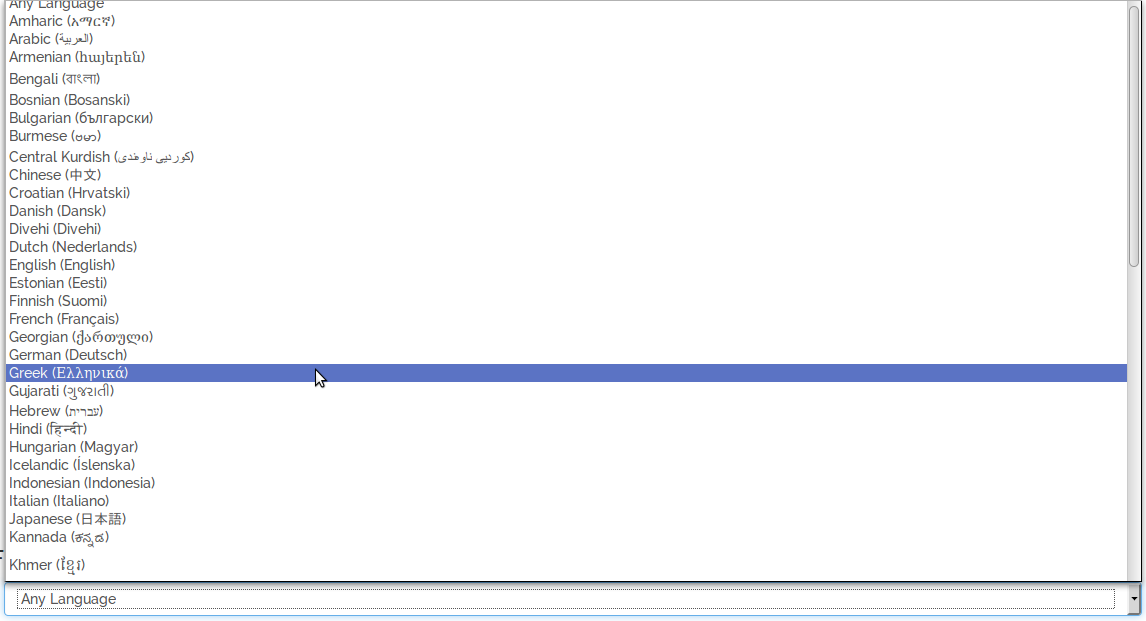
\includegraphics[width=\textwidth]{figures/languages-selection.jpg}}
\vspace{-20pt}
\caption{selection of a Tweets' language in GeoTwit}
\end{center}
\end{figure}

Since this languages' drop-down menu is located both in the dynamic and static modes, and for scalability issues, the languages list is stored as a Json format, located in the \emph{/public/data/languages.json} file. It is then loaded in the "loadLanguagesList()" function of the JavaScript file. The Json file is composed of an array of languages, in which each element have a "value" (the BCP 47 language identifier ("en", "fr", etc.) sent to the Twitter's API) and a "text" (the displayed text) attributes.\\

The identification of a tweet's language\cite{MitjaTrampus2015} seems to be performed by keywords analysis. However, since tweets' content can be very short, it may be difficult to properly determine the true language:
\begin{figure}[H]
\vspace{-5pt}
\begin{center}
\fbox{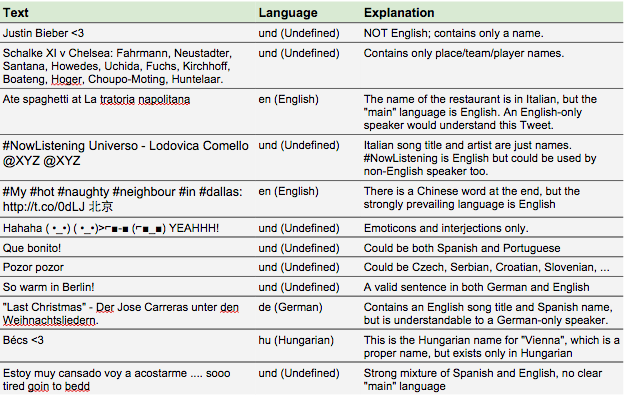
\includegraphics[width=\textwidth]{figures/langid_examples_table.png}}
\vspace{-20pt}
\caption{example of difficulties that the language-identification algorithm can encounter\cite{MitjaTrampus2015}}
\end{center}
\end{figure}

The algorithm also seems to learn from human-identified languages with sets of tweets.

\subsubsection{Selection of the Area(s) in the Search Page}
In both the streaming and the static modes of the application, the user has to choose an area in where the Tweets will be searched. In the streaming mode, he has the choice to either select a default area in a given list of countries or draw a rectangle area by drag-and-dropping the cursor on the map. In the static mode, the user can only select a circle area by drag-and-dropping the cursor, since the Twitter's Rest API asks for a circle and since it would be tricky to calculate a bounding circle of the complex polygon representing a country.\\

\emph{Selection of a default area in the list of countries}\\
As a reminder (see the prototype application's
% MIGUEL TODO - LET THIS ONE AS A REMINDER FOR ME, PLEASE :p %
"Leaflet - Countries' Border" chapter above), the country the user selects in the drop-down menu contains a value corresponding to the English name of the country. As soon as a country is selected, the JavaScript code of the "selectCountryOnMap(...)" function reads and converts to Json the "TM\_WORLD\_BORDERS-0.3" Shapefile\footnote{https://en.wikipedia.org/wiki/Shapefile}, which contains all the borders of almost each country of the worlds (note that this file is also read to add the different possible countries in the drop-down menu at the loading of the page, in the "loadCountriesList()" function). Then, the algorithm seeks for the selected country in the Json-converted data, and uses the related coordinates to draws the polygon and the map. The client also sends the server the coordinates of a rectangle bounding the selected country's territories (since a country can have many, like France with the France and Corsica territories) as said before (see the "readyToStream" web socket's type). The coordinates of this bounding rectangle are calculated in the "selectCountryOnMap(...)" function: if the country only have one territory (like Switzerland), the algorithm just selects the maximum and minimum latitude and longitude points of the polygon representing the country; if it has many territories, the algorithm selects the maximum and minimum coordinates of all the territories. The server will then search for Tweets located inside this rectangle, and send them to the client.\\

\emph{Manual selection of a rectangle/circle}\\
The code of this solution is contained in the \emph{/public/javascripts/search.js} file, specifically in the "loadSearchMap()" function. In order to be able to draw a rectangle/circle on the map by drag-and-dropping it, the \emph{w8r}'s "Leaflet.draw.drag" library\footnote{https://github.com/w8r/Leaflet.draw.drag} is used. This library uses itself the Leaflet's "Leaflet.draw" library\footnote{https://github.com/Leaflet/Leaflet.draw}, which adds support for drawing and editing polygons on Leaflet maps. Note that these libraries are NPM packages, and are thus used with the "browserify" package.\\\\
In the code, right after the map's initialization, three objects are set: the first one will contain the drawn items, and the two last ones will contain draw control's objects:
\begin{enumerate}
	\item \emph{drawnItems}: this object is added to the map as a feature group and will contain the drawn rectangle/circle.
	\item \emph{drawnControlFull[mapId]}, where "mapId" is the ID (either "streaming" or "static") of the current results' map: this object represents a toolbar that allows the user to draw a rectangle/circle on the map and which is located on the top-left of the map element. It is the default drawn control that appears when there is no polygon drawn, and is hidden as soon as the user drew one.
	\begin{figure}[H]
	\vspace{-5pt}
	\begin{center}
	\fbox{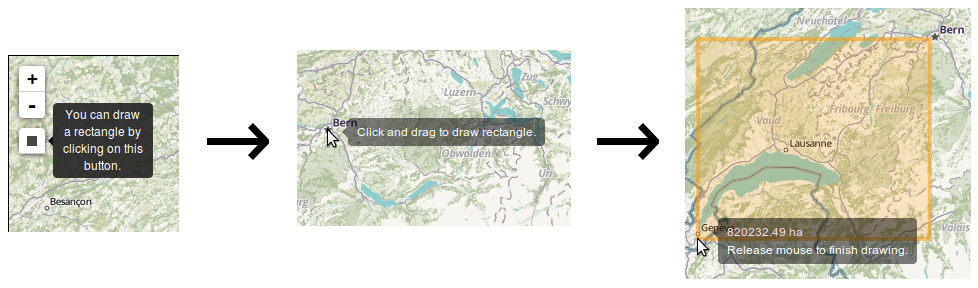
\includegraphics[width=0.86\textwidth]{figures/rectangle-drawing.jpg}}
	\vspace{-5pt}
	\caption{drawing of a rectangle on the dynamic map}
	\end{center}
	\end{figure}
	\vspace{-20pt}
	\newpage
	
	\item \emph{drawnControlEditOnly[mapId]}: this object represents another toolbar that allows the user to update the drawn rectangle/circle. It only appears when the polygon has been drawn.
	\begin{figure}[H]
	\vspace{-5pt}
	\begin{center}
	\fbox{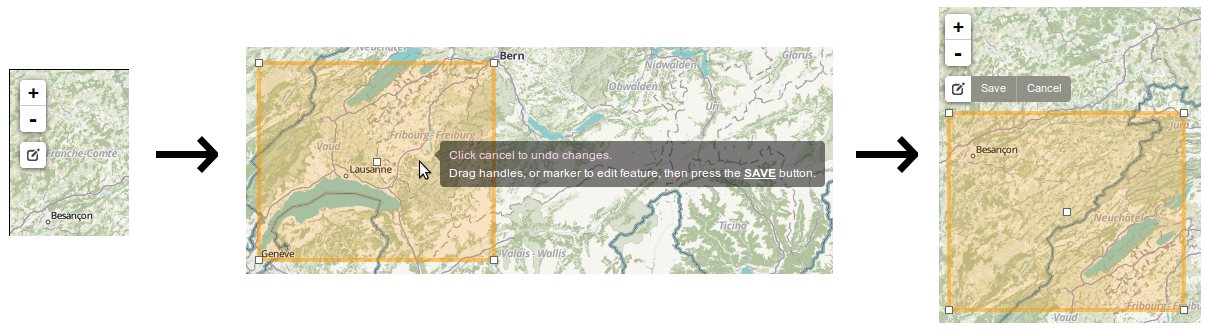
\includegraphics[width=0.86\textwidth]{figures/rectangle-edition.jpg}}
	\vspace{-5pt}
	\caption{edition of the rectangle on the dynamic map}
	\end{center}
	\end{figure}
	\vspace{-20pt}
\end{enumerate}

As soon as the user draws or edits a rectangle or a circle, the new coordinates are respectively saved in the "boundingRectangleLatLngs" object (the latitude and longitude coordinates of each corner) or in the "circleLatLngRad" (the latitude and longitude of the circle's center' point and the radius in kilometers) object, which will be sent to the server.
\bigskip

\subsubsection{Grouping of the Tweets on the Map}
Since there can be a lot of displayed Tweets on the map, they have to be grouped by clusters. Fortunately, the Leaflet library offer a plug-in for its library, called "Leaflet.markercluster"\footnote{https://github.com/Leaflet/Leaflet.markercluster}, and allowing the developer to easily group markers on a map by creating cluster groups.\\\\
In GeoTwit, only one cluster group is created (at the initialization of the results maps, in the "loadResultsMap" function):
\begin{figure}[H]
\vspace{-5pt}
\begin{center}
\fbox{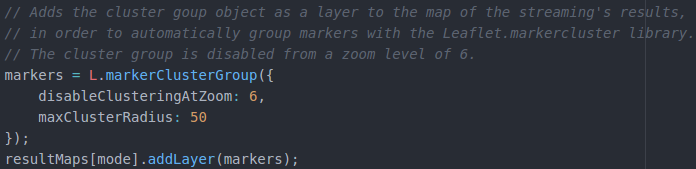
\includegraphics[width=\textwidth]{figures/cluster-group-creation.jpg}}
\vspace{-20pt}
\caption{creation of the cluster group in GeoTwit}
\end{center}
\end{figure}

The developer then just has to add a marker in this cluster group in order to make the library automatically manage the grouping.\\\\
Once a new Tweet is received, the client adds it to the cluster group if it belongs to the area; if it is not in the area, the client just ignores it.
\begin{figure}[H]
\vspace{-5pt}
\begin{center}
\fbox{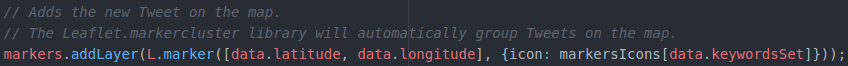
\includegraphics[width=\textwidth]{figures/tweet-adding-in-cluster-group.jpg}}
\vspace{-20pt}
\caption{adding of a Tweet in the cluster group, in GeoTwit}
\end{center}
\end{figure}

\subsection{Streaming Mode}
\subsubsection{Interface of the Streaming Process' Results}
During the streaming process, the user can accesses many information, among which:
\begin{itemize}
	\item The elapsed time since the beginning of the streaming process, updated in the "speedInterval" timer object, which is itself initialized in the "loadStreamingResultsComponents()" function called when the client received the "successfulInit" web socket type.
	\item The human-comprehensive queries (for example "dog \underline{AND} (eat \underline{OR} drink)"), generated in the "getAndFormatKeywords(...)" function (see the "\nameref{buildingTwitterQueryString}" chapter) when the client sent the user's parameters to the server.
	\item The map displaying all the received Tweets located in the selected area (see the "\nameref{receptionOfTweetsFromTheServer}" chapter below).
	\item Various charts allowing the user to better analyse the current streaming process and the data related to it (see the "\nameref{charts}" chapter below).
	\item The content of the last 100 received Tweets; this number can be changed with the "MAX\_DISPLAYED\_TWEETS" constant variable.
	\item The total number of received Tweets with geolocation tags, which corresponds to the "nbReceivedTweets" variable.
	\item The average speed of received Tweets per minute, which is calculated each second by the "speedInterval" timer object (just like the elapsed time information). The calculation is very simple and just divides the number of received Tweets by the elapsed time, then multiply it by 60 (in order to obtain minutes) and round it with two decimals.
The tricky part of the algorithm is that it also calculates the color value of the speed text (which is green when the current speed is good, and red when it is not - the goodness of the speed being determined by the "GOOD\_SPEED" constant value). The algorithm indeed calculates the hue (between "$0\to$ red" and "$120\to$ green") and the lightness values (between 50\% for the bad speed and 25\% for the good speed) of an HSL color\footnote{http://www.w3schools.com/colors/colors\_hsl.asp}, by the calculated speed per minute.
	\begin{figure}[H]
	\centering
	\begin{minipage}{0.45\textwidth}
	\centering
	\fbox{
\includegraphics[width=\textwidth]{figures/speed-color-example-1.jpg}}
	\vspace{-20pt}
	\caption{first example of speed's color}
	\end{minipage}\hfill
	\begin{minipage}{0.45\textwidth}
	\centering
	\fbox{
\includegraphics[width=\textwidth]{figures/speed-color-example-2.jpg}}
	\vspace{-20pt}
	\caption{second example of color}
	\end{minipage}
	\end{figure}
\end{itemize}

The "speedInterval" timer is stopped when the user clicks on the "Stop Streaming" button.\\\\
If the user filled the two keywords sets, the data related to the first one (human-comprehensive query, markers on the map, curves of the charts, number of received Tweets, average speed's label, content of the Tweets, etc.) will appear in \color{blue}blue\color{black}, while the ones related to the second one will appear in \color{Orange}orange\color{black}. Be careful not to confuse the subject's colors with the cluster groups' colors, which appear in green when there is not a lot of Tweets in the group, and in red when there is a lot of Tweets.
\begin{figure}[H]
\vspace{-5pt}
\begin{center}
\fbox{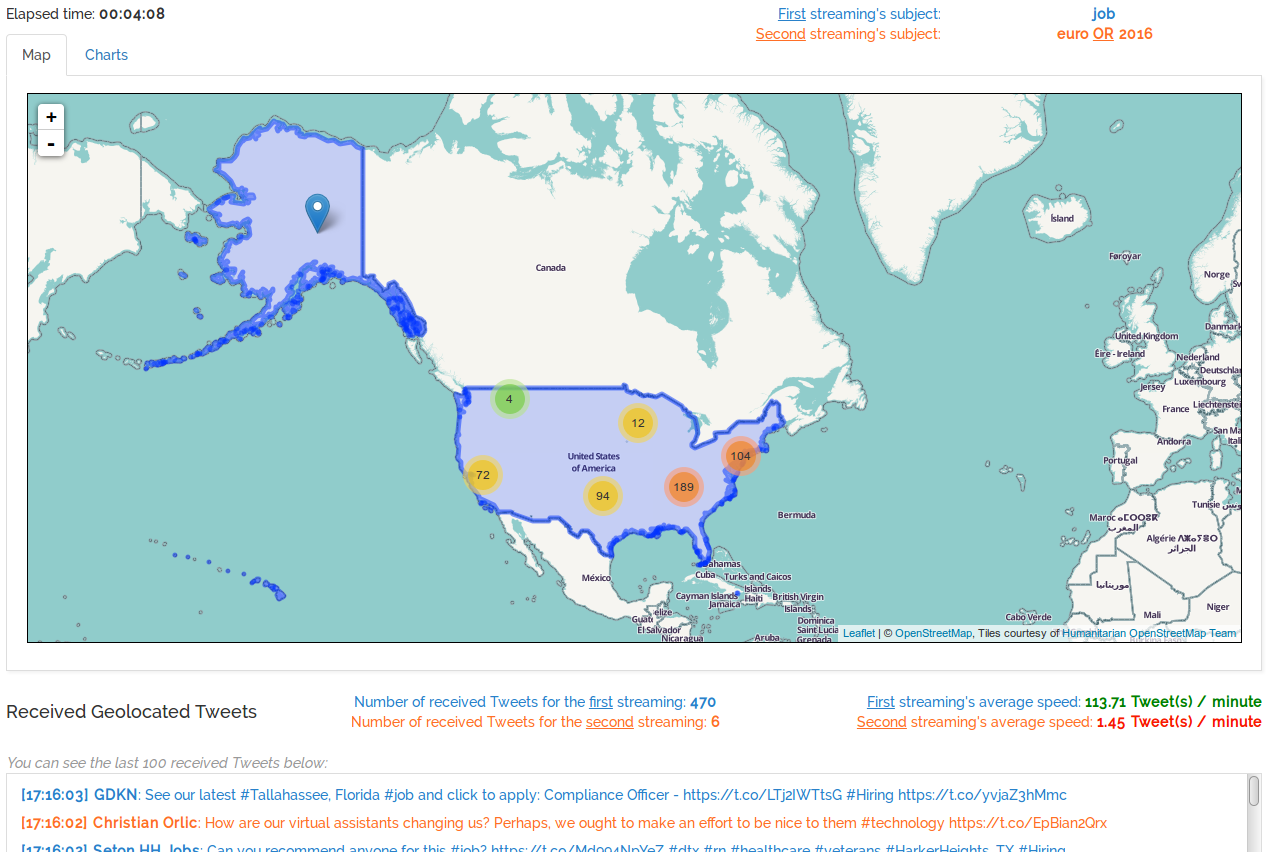
\includegraphics[width=\textwidth]{figures/streaming-interface-example.jpg}}
\vspace{-20pt}
\caption{example of an interface of the streaming process' results}
\end{center}
\end{figure}
\vspace{-10pt}

Charts are properly explained in the "\nameref{charts}" chapter below.
\bigskip

\subsubsection{Reception of Tweets from the Server}
\label{receptionOfTweetsFromTheServer}
Once the streaming process started, the client first draws the saved selected area (either the rectangle or the complex polygon bounding the area or country). When the server received a Tweet matching the filter, the language and the bounding rectangle, it sends it to the client. Once the client received the "newTweet" web socket message, it first saves the total number of received Tweets (both with or without geolocation) contained in the web socket's content, then acts according to the selected location's type (determined by a boolean variable set when the user selected an area):
\begin{itemize}
	\item If the user manually selected a rectangle area on the map, it means that the received Tweet necessarily is in the selected area, so the client just displays it on the map and in the received Tweets panel (with the "addTweetOnPage(...)" function). It also increments the local number of received Tweets, in order to properly calculate the average reception's speed.
	\newpage
	\item It is more complicated if the user selected an default area from the drop-down menu: since the server indeed searched for Tweets within the bounding rectangle, some of the received Tweets may not be in the selected area.
	\begin{figure}[H]
	\vspace{-5pt}
	\begin{center}
	\fbox{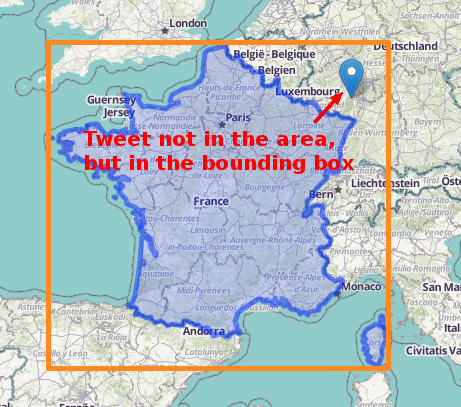
\includegraphics[width=0.86\textwidth]{figures/tweet-located-in-the-bounding-box-but-not-in-the-polygon.jpg}}
	\vspace{-5pt}
	\caption{example of a Tweet located in the bounding box of the selected country's territories, but not in the territories themselves}
	\end{center}
	\end{figure}
	\vspace{-20pt}
	
	In this case, the client must check that the received Tweet belongs to the complex polygon. In order to properly accomplish this task, the Point Inclusion in Polygon algorithm (\emph{PNPOLY})\cite{RandolphFranklin2016} was used with an updated version of the \emph{substack}'s "point-in-polygon" library found on GitHub\footnote{https://github.com/substack/point-in-polygon/blob/master/index.js}, which allows the developer to determinate if a given point is in a given polygon. Since the \emph{PNPOLY} algorithm is well explained in the given web site, it will not be totally explained again here. Here is still some of the important points: according to the documentation, the algorithm runs a semi-infinite ray horizontally (increasing x, fixed y) out from the test point, and count how many edges it crosses. At each crossing, the ray switches between inside and outside. This is called the Jordan curve theorem. The case of the ray going through a vertex is handled correctly via a careful selection of inequalities. The ray is tested against each edge to determinate if the point is in the half-plane to the left of the extended edge and if the point's Y coordinate is within the edge's Y-range.
\end{itemize}
\newpage

\subsubsection{Charts}
\label{charts}
In order to draw charts in GeoTwit, the Chart.js library is used\footnote{http://www.chartjs.org/}. There are several other well-known libraries (like D3.js\footnote{https://d3js.org/}), but they are either too complicated for the simple uses of the application or not as user-friendly and as documented as Chart.js.\\\\
In GeoTwit, there are six possible charts, ordered in two categories: Tweets having geolocation tags, and all Tweets (both with or without geolocation tags). The following screenshots were taken during a example test made with the \color{blue}"job" (blue) \color{black}and \color{Orange}"euro \underline{OR} 2016" (orange) \color{black}keywords sets and located in the U.S.A.
\begin{enumerate}
	\item Charts related to \textbf{Tweets \underline{having} geolocation tags}:
	\begin{enumerate}
		\item \textbf{Total of received Tweets, by time}: this "line" chart displays the total of received Tweets that have a geolocation tag, first by seconds, and then be minutes once 60 seconds elapsed.
		\begin{figure}[H]
		\vspace{-5pt}
		\begin{center}
		\fbox{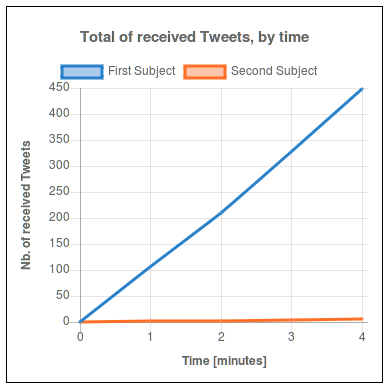
\includegraphics[width=0.37\textwidth]{figures/gtrt-example.jpg}}
		\vspace{-5pt}
		\caption{example of the "GTRT" chart}
		\end{center}
		\end{figure}
		\vspace{-10pt}
		
		\item \textbf{Reception of Tweets, by time}: this "line" chart displays the number of received Tweets during time periods (first by seconds, and then be minutes once 60 seconds elapsed).
		\begin{figure}[H]
		\vspace{-5pt}
		\begin{center}
		\fbox{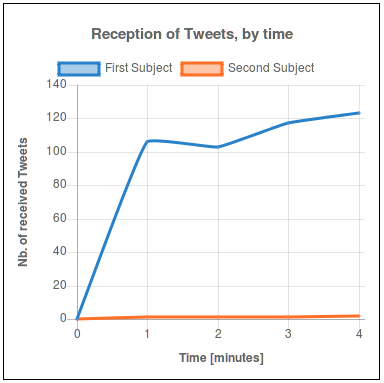
\includegraphics[width=0.37\textwidth]{figures/grt-example.jpg}}
		\vspace{-5pt}
		\caption{example of the "GRT" chart}
		\end{center}
		\end{figure}
		\vspace{-10pt}
		
		\item \textbf{Parts of the received Tweets by subject}: this "doughnut" chart compares the part of received Tweets for each subject, and is only visible when the user filled the two keywords sets.
		\begin{figure}[H]
		\vspace{-5pt}
		\begin{center}
		\fbox{\includegraphics[width=0.45\textwidth]{figures/gprt-example.jpg}}
		\vspace{-5pt}
		\caption{example of the "GPRT" chart}
		\end{center}
		\end{figure}
		\vspace{-10pt}
	\end{enumerate}
	
	\item Charts related to all kinds of Tweets (\textbf{with and \underline{without} geolocation tags}):
	 \begin{enumerate}
	 	\item \textbf{Total of received Tweets, by time}: this "line" chart displays the total of all received Tweets (that have or not a geolocation tag), first by seconds, and then be minutes once 60 seconds elapsed.
	 	\begin{figure}[H]
		\vspace{-5pt}
		\begin{center}
		\fbox{\includegraphics[width=0.45\textwidth]{figures/atrt-example.jpg}}
		\vspace{-5pt}
		\caption{example of the "ATRT" chart}
		\end{center}
		\end{figure}
		\vspace{-10pt}
		\newpage		
		
		\item \textbf{Reception of Tweets, by time}: this "line" chart displays the number of all received Tweets (that have or not a geolocation tag) during time periods (first by seconds, and then be minutes once 60 seconds elapsed).
		\begin{figure}[H]
		\vspace{-5pt}
		\begin{center}
		\fbox{\includegraphics[width=0.45\textwidth]{figures/art-example.jpg}}
		\vspace{-5pt}
		\caption{example of the "ART" chart}
		\end{center}
		\end{figure}
		\vspace{-10pt}
		
		\item \textbf{Tweets with geolocation vs. Tweets without}: this "bar" chart displays the percentage of Tweets that have a geolocation tags versus the percentage of those which do not have one.
		\begin{figure}[H]
		\vspace{-5pt}
		\begin{center}
		\fbox{\includegraphics[width=0.45\textwidth]{figures/agvw-example.jpg}}
		\vspace{-5pt}
		\caption{example of the "AGVW" chart}
		\end{center}
		\end{figure}
		\vspace{-10pt}
	 \end{enumerate}
\end{enumerate}

All these charts are responsive and react when the user moves the mouse over their elements.
\newpage

Since the documentation of the library is well documented, everything will not be explained here; the initialization of the charts and the timers related to their refreshment is located in the "loadStreamingResultsCharts(...)" function. Firstly, the contexts of the charts (the HTML elements) are initialized, then the empty datasets of the charts and the charts themselves. The interesting parts of the algorithm concern the refreshment of the charts; there are two timers refreshing the charts each second (and then each minute for the first one): 
\begin{enumerate}
	\item \textbf{lineChartsUpdateInterval}: this timer refreshes all the "line" charts (so 4 on the 6 charts) each second, and then each minute when 60 seconds elapsed. All the data are calculated with the "nbReceivedTweets" and "lastNbReceivedTweets" objects, which respectively contain the total number of received Tweets (for the Tweets with geolocation and for all the Tweets) and the last number of received Tweets that were calculated during the last tick of the timer.
	\item \textbf{doughnutBarChartsUpdateInterval}: this timer refreshes the "doughnut" and "bar" charts each second. All the data are calculated with the "nbReceivedTweets" object. The "bar" chart contains two dataset in case of multiple keywords sets (one for each keywords set), in order to display the two subjects' colors. Each data set contains 4 values (2 for the current subject and two null value for the other subject), in order to only display 4 bars (and not 8: \emph{2 subjects x 4 bars}).
\end{enumerate}

Once the charts are initialized, the timers are started. They are stopped when the user clicks on the "Stop Streaming" button.

\subsection{Static Mode}
\subsubsection{Selection of the Dates}
In the static mode, the user has to select the search's start and end dates in the \emph{YYYY-MM-DD} format. Since the Twitter's REST API only allows the developers to get Tweet from a maximum of 9 days ago, the user cannot select dates that do not fit this filter.\\\\
In order to facilitate the selection of dates, the \emph{amsul}'s date picker "pickadate.js" library\footnote{https://github.com/amsul/pickadate.js} is used, with the "classic" theme. This library is located in the \emph{public/javascripts} folder in the "picker.min.js", "picker.date.min.js" and the "legacy.js" (this last one is used for older versions of Internet Explorer) files.\\\\
The date picker is loaded on dates fields as soon as the Search page successfully loaded.
\begin{figure}[H]
\vspace{-5pt}
\begin{center}
\fbox{\includegraphics[width=0.7\textwidth]{figures/date-picker-loading.jpg}}
\vspace{-5pt}
\caption{loading of the date picker on the dates fields}
\end{center}
\end{figure}
\vspace{-10pt}
\newpage

\subsubsection{Retrieval of Tweets with the Server}
\label{retrievalOfTweets}
Once the user properly filled all the fields, the client sends an Ajax request to the server, in order to retrieve the results. This Ajax request is located in the "getStaticTweets()"method of the \emph{search.js} file. The following parameters are sent in a Json format:
\begin{itemize}
	\item \textbf{firstKeywords}: the first keywords set filled by the user, formatted with the "getAndFormatKeywords(...)" function (see the "\nameref{buildingTwitterQueryString}" chapter above).
	\item \textbf{secondKeywords}: the second formatted keywords set filled by the user (it can be empty).
	\item \textbf{fromDate}, \textbf{toDate}: the \emph{YYYY-MM-DD} formatted dates from and to where the Tweets will be searched.
	\item \textbf{locationLat}, \textbf{locationLon}, \textbf{locationRad}: the latitude and longitude coordinates of the circle's middle point, and the radius of the circle in kilometers.
	\item \textbf{language}: the BCP 47 language identifier of the search's language.
\end{itemize}

Once the server responded to the Ajax request with Json, the response message can contain either an error (in this case, the client just displays an error message) or the list of Tweets. Since there can be a lot of Tweets, the data transfer can take a while, so the search button changes its display:
\begin{figure}[H]
\vspace{-5pt}
\begin{center}
\fbox{\includegraphics[width=\textwidth]{figures/search-button.jpg}}
\vspace{-20pt}
\caption{display of the search button when the user clicked on it 
in order to search for Tweets}
\end{center}
\end{figure}
\vspace{-10pt}

Once the Tweets lists have been received, the client first calculates the numbers of Tweets, then concatenates the lists (since there is one list per keywords set), sorts the new-created list by the dates and times of the Tweets, then adds each Tweet one by one on the results map (only for the Tweets having a geolocation tag) with the "addTweetOnPage(...)" function, and adds each Tweet in the Tweets panel.\\\\
The Tweets are also grouped with cluster groups, like in the streaming mode's results (see the "\nameref{receptionOfTweetsFromTheServer}" chapter below).
\bigskip

\subsubsection{Interface of the Static Mode's Results}
Once the static search is done, the user can accesses many information, among which:
\begin{itemize}
	\item The human-comprehensive queries (for example "dog \underline{AND} (eat \underline{OR} drink)"), generated in the "getAndFormatKeywords(...)" function (see the "\nameref{buildingTwitterQueryString}" chapter) when the client sent the user's parameters to the server.
	\item The map that displays all the Tweets located in the selected area. Note that some Tweets can be displayed outside the circle, due to the search algorithm of the Twitter's REST API, which is a little tricky.
	\item The content of the all the Tweets.
	\item The total number of received Tweets, both with and without geolocation tags.
\end{itemize}
\newpage

If the user filled the two keywords sets, the data related to the first one will appear in \color{blue}blue\color{black}, while the ones related to the second one will appear in \color{Orange}orange\color{black}.
\begin{figure}[H]
\vspace{-5pt}
\begin{center}
\fbox{\includegraphics[width=\textwidth]{figures/static-mode-interface.jpg}}
\vspace{-20pt}
\caption{example of the interface of the static mode's results}
\end{center}
\end{figure}
\vspace{-10pt}

\chapter{Tests}
This chapter contains all the the documentation related to the application's tests.\\
A Twitter account was specially created for this project and has been used for most of these tests:
\begin{itemize}
	\item \textbf{Username}: GeoTwitHeig
	\item \textbf{Password}: @heigVdRocks42
\end{itemize}
Feel free to use these credentials for your own tests.

\section{Functional Tests}
All the development process and thus the functional tests were processed with the version 47.0 of Firefox on Linux Mint. Though, other web browser were tested in the "\nameref{webBrowsersCompatibilities}" chapter above.

\begin{center}
\def\arraystretch{1.5}
\begin{longtable}{|l|p{10cm}|p{4.4cm}|}\hline
	\textbf{\#} & \textbf{Description} & \textbf{Results}\\\hline \endhead
	\multicolumn{3}{|c|}{\textbf{Miscellaneous}}\\\hline
	1 & If the user tries to access an non-existent page, a "Not Found" page is displayed. & \color{ForestGreen}OK\color{black}\\\hline
	2 & The user can access the about and help pages, regardless of whether he is connected or not. & \color{ForestGreen}OK\color{black}\\\hline
	3 & The web site's GUI is stable. & \color{ForestGreen}OK\color{black}\\\hline
	4 & The web site's GUI is responsive. & \color{Orange}Only for desktop applications\color{black}\\\hline	
	5 & Maps are responsive and allow the user to zoom in and out and to move around the world by drag-and-dropping the content. & \color{ForestGreen}OK\color{black}\\\hline
	
	\multicolumn{3}{|c|}{\textbf{Home page and connection process}}\\\hline
	6 & The user can properly access the application's home page if he is disconnected. & \color{ForestGreen}OK\color{black}\\\hline
	7 & If the user is not connected and try to access pages different than the home page, he is redirected on the home page with an error message. & \color{ForestGreen}OK\color{black}\\\hline
	8 & The user can access the Twitter's authentication page by clicking either on the "Get Started" or on the "Connect" button. & \color{ForestGreen}OK\color{black}\\\hline
	9 & If the user denied the authentication process or if an error occurred, he is properly redirected on the home page with an explicit error message. & \color{ForestGreen}OK\color{black}\\\hline
	10 & Once the user successfully connected, he is able to navigate through the web site and to access the tools. He is however redirected to the search page if he tries to access the home page. & \color{ForestGreen}OK\color{black}\\\hline
	11 & If the connected user clicks on the "Disconnect" button, he is properly disconnected, the session is entirely destroyed and he cannot access search pages anymore. & \color{ForestGreen}OK\color{black}\\\hline
	12 & The session lasts 7 days and the user is not disconnected before this time limit, \underline{except if a modification was done in} \underline{the server's code}. & \color{ForestGreen}OK\color{black}\\\hline
	
	\multicolumn{3}{|c|}{\textbf{Main Search Page}}\\\hline		
	13 & The user is redirected on the main search page if he clicks on the GeoTwit's logo located on the header bar & \color{ForestGreen}OK\color{black}\\\hline
	14 & The user can navigate through both the dynamic and static modes with the tab system. & \color{ForestGreen}OK\color{black}\\\hline
	
	\multicolumn{3}{|c|}{\textbf{Dynamic Mode - Files Importation}}\\\hline		15 & By clicking on the importation button, a pop-up window that allows the user to select a file appears. & \color{ForestGreen}OK\color{black}\\\hline
	16 & If the user select a wrong type of file (i.e. an image), an error is displayed. & \color{ForestGreen}OK\color{black}\\\hline
	17 & If the selected file is an empty text file, an error is displayed. & \color{ForestGreen}OK\color{black}\\\hline
	18 & If the selected file's content is not a valid GeoTwit content, an error is displayed. & \color{ForestGreen}OK\color{black}\\\hline
	19 & During the importation of the file, a progress-bar is displayed and is automatically refreshed. & \color{ForestGreen}OK\color{black}\\\hline
	20 & Once the importation was successfully done, the user is redirected on the result page and can access the information. & \color{ForestGreen}OK\color{black}\\\hline
	21 & The information displayed are the same as the ones contained in the file and thus the imported ones. & \color{ForestGreen}OK\color{black}\\\hline
	
	
	\multicolumn{3}{|c|}{\textbf{Dynamic Mode - Fields Validation}}\\\hline	
	22 & The user cannot write more than 60 characters in the keywords sets' fields. & \color{ForestGreen}OK\color{black}\\\hline
	23 & If the user tries to bypass the characters limitation by editing the text field's properties, the server still displays an error message. & \color{ForestGreen}OK\color{black}\\\hline
	24 & If the user did not set at least one keywords set when clicking on the "Start Streaming" button, an error message appears. & \color{ForestGreen}OK\color{black}\\\hline
	25 & The countries included in the default area list are listed in alphabetical order. & \color{ForestGreen}OK\color{black}\\\hline
	26 & If the user did not either choose a default area in the countries' list or manually draw a rectangle on the map, an error message is displayed. & \color{ForestGreen}OK\color{black}\\\hline
	27 & The user is able to draw only one rectangle on the map and is also able to update it. & \color{ForestGreen}OK\color{black}\\\hline
	28 & If a rectangle is drawn or it the user selected a country, all existing polygons are removed from the map. & \color{ForestGreen}OK\color{black}\\\hline
	29 & The languages list contains all the possible languages in alphabetic order. & \color{ForestGreen}OK\color{black}\\\hline
	30 & Once all fields are valid, the user is properly redirected to the results page. & \color{ForestGreen}OK\color{black}\\\hline
	31 & When the user clicks on the button and everything is valid, the server properly removes the current user's existing file-to-export in its side, if there was one. & \color{ForestGreen}OK\color{black}\\\hline
	
	\multicolumn{3}{|c|}{\textbf{Dynamic Mode - Results Page}}\\\hline	
	32 & The results page's components are properly loaded once the user accessed it. & \color{ForestGreen}OK\color{black}\\\hline
	33 & If the user only filled one subject, only the blue components are displayed and enabled. & \color{ForestGreen}OK\color{black}\\\hline
	34 & If the user filled two subjects, the orange components also appears and are enabled. & \color{ForestGreen}OK\color{black}\\\hline
	35 & The displayed information correspond to the ones the user filled. & \color{ForestGreen}OK\color{black}\\\hline
	36 & The elapsed time's timer is enabled and working. & \color{ForestGreen}OK\color{black}\\\hline
	37 & The user can switch between the map and the charts by using the tab system of the page. & \color{ForestGreen}OK\color{black}\\\hline 
	38 & Tweets are received in the selected location only. & \color{ForestGreen}OK\color{black}\\\hline
	39 & The average speed is correctly refreshed and changes its color according to the speed (green if good, red if bad). & \color{ForestGreen}OK\color{black}\\\hline
	40 & Once a tweet is received, it is correctly displayed on the map and in the tweets panel below with the right color, and the number of received tweet is updated. & \color{ForestGreen}OK\color{black}\\\hline
	41 & Only the last 100 received tweets are displayed in the tweets panel below & \color{ForestGreen}OK\color{black}\\\hline
	42 & Group clusters are properly working and disappear once the user zoomed at a zoom level of 8 or more. & \color{ForestGreen}OK\color{black}\\\hline
	43 & There is 5 available charts if the user entered only one subject, and 6 otherwise. & \color{ForestGreen}OK\color{black}\\\hline
	44 & The charts are correctly refreshed each second, then each minute once 60 seconds passed. In addition, they correctly differentiate the subjects if the user filled two subjects. & \color{ForestGreen}OK\color{black}\\\hline
	45 & The charts are decent, correct, and responsive. & \color{ForestGreen}OK\color{black}\\\hline
	46 & The streaming process is stopped once the user clicked on the "Stop Streaming" button, a new "Make a new search" button appears, and an exportation pop-up is instantaneously displayed. & \color{ForestGreen}OK\color{black}\\\hline
	47 & If the user either clicked the "Cancel" button of the pop-up window or closed it, the file is removed from the server side. & \color{ForestGreen}OK\color{black}\\\hline
	48 & If the user clicked the "Ok" button, he is able to save the file-to-export wherever he wants on his computer, then the file is removed from the server side. He is then able to export this file from the main search page. & \color{ForestGreen}OK\color{black}\\\hline
	49 & Once the user clicked on the "Make a new search" button, he is redirected on the main search page. & \color{ForestGreen}OK\color{black}\\\hline
	 
	\multicolumn{3}{|c|}{\textbf{Static Mode - Fields Validation}}\\\hline
	50 & The keywords sets fields act like the dynamic mode's ones. & \color{ForestGreen}OK\color{black}\\\hline
	51 & The user can only select dates between the current date and the date it was 9 days ago. & \color{ForestGreen}OK\color{black}\\\hline
	52 & If the date are either not set or not valid, an error message is displayed. & \color{ForestGreen}OK\color{black}\\\hline
	53 & An error message is displayed if the user did not select a circle area on the map. & \color{ForestGreen}OK\color{black}\\\hline
	54 & The user is able to draw only one circle on the map and is able to update it. & \color{ForestGreen}OK\color{black}\\\hline
	55 & The languages list contains all the possible languages in alphabetic order. & \color{ForestGreen}OK\color{black}\\\hline
	56 & Once all the fields are valid, the user can search for results by clicking on the "View Results!" button. & \color{ForestGreen}OK\color{black}\\\hline
	57 & The button changes of behavior during the search process. & \color{ForestGreen}OK\color{black}\\\hline
	58 & If there was no result, a pop-up message is displayed. & \color{ForestGreen}OK\color{black}\\\hline
	59 & If the user exceeded the limit of requests made, a pop-up message is displayed. & \color{ForestGreen}OK\color{black}\\\hline
	60 & If there was no error, the user can access the results page. & \color{ForestGreen}OK\color{black}\\\hline
	 
	\multicolumn{3}{|c|}{\textbf{Static Mode - Results Page}}\\\hline
	61 & The results page act like the dynamic mode's result page, except that the user cannot access charts and everything is fixed. & \color{ForestGreen}OK\color{black}\\\hline
	62 & The tweet panel has no number limit and displays the tweets both with and without geolocation tags. & \color{ForestGreen}OK\color{black}\\\hline
	63 & Tweets are received in the selected location only. & \color{Orange}Certain tweets are displayed outside the circle, but this issue is apparently due to the Twitter's algorithm, which is tricky.\color{black}\\\hline
\end{longtable}
\end{center}
\vspace{-20pt}

All tests thus successfully passed, except the \#4 one, which was thus not specified in the specifications.

\subsection{Web Browsers - Compatibilities}
\label{webBrowsersCompatibilities}
As mentioned above, all the development process and thus the functional tests were processed with the version 47.0 of Firefox on Linux Mint.\\\\
Since the end users can have different operating systems and/or web browsers, the functional tests' list was also tested with a variety of combinations. Here is the obtained results:
\begin{center}
\def\arraystretch{1.5}
\begin{longtable}{|l|l|l|p{7cm}|}\hline
	\textbf{\#} & \textbf{Operating System} & \textbf{Web Browser} & \textbf{Results}\\\hline \endhead
	1 & Linux Mint & Mozilla Firefox 47 & \color{ForestGreen}OK\color{black}\\\hline
	2 & Linux Mint & Chromium 51 & \color{ForestGreen}Some components' borders are missing.\color{black}\\\hline
	3 & Windows7 & Mozilla Firefox 47 & \color{ForestGreen}OK\color{black}\\\hline
	4 & Windows7 & Google Chrome 51 & \color{ForestGreen}Some components' borders are missing.\color{black}\\\hline
	5 & Windows7 & Internet Explorer 11 & \color{ForestGreen}The font of the home page's title is not loaded; certain components  (like charts) are either too big or too small; some little bugs of interface.\color{black}\\\hline	
\end{longtable}
\end{center}
\vspace{-20pt}

In summary, all other recent web browsers seem to be able to run the application (sometimes with small bugs of interface, but nothing to worry about).
\newpage

In order to make Internet Explorer work with the application, the default parameters values of the JavaScript function had to be removed, since this web browser does not seem to properly follow the JavaScript's ES6/ES2015 norms. Also, in order to make the file importation work with this "browser", the "uploadAndParse" action of the \textbf{SearchController} now also valid the "text/plain" file's content type (used by IE) in addition to the basic "application/octet-stream" used by all other browsers.

\section{Load Tests}
Two load tests types were done:
\begin{enumerate}
	\item \textbf{Tests about the number of received tweets}: these tests are used to analyze the application's reaction when there is a huge amount of data to process, display and/or import.\\\\
	The \underline{static mode} is easy to test here: indeed, since the number of requests is limited to 170 (about 17'000 tweets) by the application's server, we just have to find a subject that contains a number of tweet big enough to reach this limit. The "job" keyword in the U.S.A. always gave good results over the other tests, and was thus used here. Firstly, here are the obtained results:
	\begin{figure}[H]
	\vspace{-5pt}
	\begin{center}
	\fbox{\includegraphics[width=0.85\textwidth]{figures/load-tests-static-mode.jpg}}
	\vspace{-5pt}
	\caption{results of the load tests for the static mode with the "job" keyword}
	\end{center}
	\end{figure}
	\vspace{-10pt}
	
	As expected, about 17'000 tweets were received, including about 5'000 ones with geolocation tags. The search process was timed and took 1 minute and 54 seconds. The map was very fluid since the tweets were grouped by cluster groups; however, when the map was zoomed enough to disable the cluster groups (zoom level of 8 or more) in areas with high tweets densities (like the West Coast), the loading took about 10 seconds, but the map was still fluid after the process. When the groups were enabled again by zooming out, the loading took about 2 seconds. This load test was then a success.\\	
	
	Concerning the \underline{dynamic mode}, the streaming process had to run for hours in order to properly accumulate a charge wide enough. In order to get a huge amount of tweets, GeoTwit listened for the "job" and "beach" keywords sets in the U.S.A. (since there is a huge amount of tweets posted with geolocation tags for these subjects in general) for 13 hours and 30 minutes between 21:00 on 26.07.2016 and 10:30 on 27.07.2016. Firstly, here are the obtained results:
	\begin{figure}[H]
	\vspace{-5pt}
	\begin{center}
	\fbox{\includegraphics[width=0.85\textwidth]{figures/load-test-streaming-map.png}}
	\vspace{-5pt}
	\caption{results' map of the streaming mode's load tests with the "job" and "beach" keywords}
	\end{center}
	\end{figure}
	\vspace{-10pt}
	
	\begin{figure}[H]
	\vspace{-5pt}
	\begin{center}
	\fbox{\includegraphics[width=0.85\textwidth]{figures/load-test-streaming-charts.png}}
	\vspace{-5pt}
	\caption{charts of the streaming mode's load tests with the "job" and "beach" keywords}
	\end{center}
	\end{figure}
	\vspace{-10pt}	
	
	The first comment we can do is about the geolocated reception, whose form is pretty logarithmic. This can be explained by the fact that it was the evening (18:00) in the U.S.A. approximately since the 180th minute, so there were less people/bots posting for jobs.\\\\
	Concerning the load tests observations, the page was still very fluid: it was possible to navigate the map and to interact with the chart without having any slowness, thanks to the cluster groups. However, zooming the map at a zoom level of 8 or more (which thus removes the cluster groups) on the area with the highest density took some time (about 40 seconds) to load the markers; once they were properly loaded, some little slowness began to appear, but the map was still well usable, though.
	
	\begin{figure}[H]
	\vspace{-5pt}
	\begin{center}
	\fbox{\includegraphics[width=0.85\textwidth]{figures/load-tests-streaming-.map-zoomed.jpg}}
	\vspace{-5pt}
	\caption{map of the load tests' results zoomed at a zoom level of 8}
	\end{center}
	\end{figure}
	\vspace{-10pt}
	
	At the end of the process, the backup file was easily exported. The importation process took about 1 minute and 42 seconds (during which the overloaded web browser displayed some "script not answering" pop-up messages), but was successful in the end. Once loaded, the reaction of the file results' map was exactly the same as the previous map.
	\bigskip
	
	\item \textbf{Tests about the number of application that simultaneously search for tweets}: since several Twitter accounts are required for properly performing these tests and it would be annoying to create these account and connect with them, only two accounts were used but with 4 different browsers in two different machines. The processes perfectly worked and there was not even a single lag.\\
	Of course, the number of applications was not wide enough to hope to get interesting reactions, but it though confirms that the server can easily manage several clients at the same time.
	
\end{enumerate}

\section{Security Tests}
% TODO

\section{Subjects Analyzed with the Streaming Mode}
\subsection{The "job" keyword}
When listening to the "job" keyword in the territories of the U.S.A., there was \underline{always} a great tweet reception (about 130 geolocated tweets / minute) at any time of day (in the U.S.A., so during the European afternoon and evening). Since the majority of these tweets always contained the same texts ("Want to work at...?", "We're hiring!", "Can you recommend anyone for this job?", "This job might be a great fit for you", "If you're looking for a job", etc.) regardless to their locations (which were almost everywhere in the territories), it was concluded that they were posted by bots per time interval. An way to guarantee the veracity of this assumption is to look at the charts generated for this keyword, which are linear in time during the day:
\begin{figure}[H]
\vspace{-5pt}
\begin{center}
\fbox{\includegraphics[width=0.5\textwidth]{figures/job-chart.jpg}}
\vspace{-5pt}
\caption{total number of received tweets by time, for the "job" subject in the U.S.A.}
\end{center}
\end{figure}
\vspace{-10pt}

This situation was very interesting throughout the application's implementation process, because it assured a way to always have data to test.

\subsection{Subjects by Countries}
This section contains analyses separated by countries. The majority of them is related to the subjects already analyzed by the prototype application in the table of the "Interesting Twitter's Subjects"
% TODO
chapter, but during hours instead of minutes. They are separated by countries.

\subsubsection{United Kingdom}
Both the "bbc" and the "london" subjects were first analyzed here at the same time, on 18.08.2016 between 15:00 and 17:00.
\begin{figure}[H]
\vspace{-5pt}
\begin{center}
\fbox{\includegraphics[width=\textwidth]{figures/analysis-uk-bbc-london-map.jpg}}
\vspace{-20pt}
\caption{analysis' map of the "bbc" and "london" keywords in UK}
\end{center}
\end{figure}
\vspace{-10pt}

\begin{figure}[H]
\vspace{-5pt}
\begin{center}
\fbox{\includegraphics[width=\textwidth]{figures/analysis-uk-bbc-london-charts.jpg}}
\vspace{-20pt}
\caption{analysis' charts of the "bbc" and "london" keywords in UK}
\end{center}
\end{figure}
\vspace{-10pt}

The "bbc" subject gave bad results for the geolocated tweets, with an average speed reception of only 0.06 tweet per minute (99.97\% of the tweets did not have geolocation data). The "london" subject was better, although not amazing either (here, 97.84\% did not have geolocation tag). It is interesting to note than the reception of all kinds of tweets of the first subject was in a "stair" shape, while the second subject's one was pretty linear, but in the end their value were very close. Thus, British people seem to be more apt to post tweets related to London than tweets related to the BBC.
\bigskip

July 19 was the \underline{hottest day of the Summer} in UK. The idea of analysing this subject came from the fact that people tend to like complaining about the weather on the social networks, in general. Indeed, by analysing the "hot" or "sun" keywords, about 370 geolocated tweets and about 160'000 tweets of all kinds were posted between 13:00 and 16:00.
\begin{figure}[H]
\vspace{-5pt}
\begin{center}
\fbox{\includegraphics[width=\textwidth]{figures/analysis-uk-hot-sun-map.jpg}}
\vspace{-20pt}
\caption{analysis' map of the "hot" or "sun" keywords in UK during the hottest day}
\end{center}
\end{figure}
\vspace{-10pt}

\begin{figure}[H]
\vspace{-5pt}
\begin{center}
\fbox{\includegraphics[width=\textwidth]{figures/analysis-uk-hot-sun-charts.jpg}}
\vspace{-20pt}
\caption{analysis' charts of the "hot" or "sun" keywords in UK during the hottest day}
\end{center}
\end{figure}
\vspace{-10pt}

About 99.77\% of the posted tweets did unfortunately not have geolocation data.


\subsubsection{Italy}
Both the "pizza" and the "roma" subjects were analyzed at the same time on 18.08.2016 between 17:00 and 19:00. Like in the prototype application's analysis, not a single tweet was received during the streaming process, so it was decided that no other test will be performed for this country.

\subsubsection{France}
The word "paris" was tested on 19.07.2016 between 17:00 and 19:00.
\begin{figure}[H]
\vspace{-5pt}
\begin{center}
\fbox{\includegraphics[width=\textwidth]{figures/analysis-france-paris-map.png}}
\vspace{-20pt}
\caption{analysis' map of the "paris" keyword in France}
\end{center}
\end{figure}
\vspace{-10pt}

\begin{figure}[H]
\vspace{-5pt}
\begin{center}
\fbox{\includegraphics[width=\textwidth]{figures/analysis-france-paris-charts.png}}
\vspace{-20pt}
\caption{analysis' charts of the "paris" keyword in France}
\end{center}
\end{figure}
\vspace{-10pt}

As expected, a lot of tweets were received from Paris, since it was the main concerned subject.\\

France was also analyzed among other countries during the final match of the Euro2016 event (see the "\nameref{euro2016final}" chapter below).

\subsubsection{Switzerland}
Switzerland is a small country, but does that mean that people do not post from there on Twitter?\\

A first analysis was made on July 20 and 21 from 21:00 to 04:00, notably during the live of Iron Maiden at the Paleo Festival of Nyon (with the "paleo" subject), and gave just one result at 22:23:
\begin{figure}[H]
\vspace{-5pt}
\begin{center}
\fbox{\includegraphics[width=\textwidth]{figures/analysis-switzerland-paleo-map.png}}
\vspace{-20pt}
\caption{analysis' map of the "paleo" keyword in Switzerland}
\end{center}
\end{figure}
\vspace{-10pt}

The second Swiss analysis was made on July 21 between 14:00 and 16:00, and was about the main Swiss industries/companies ("coop \underline{OR} glencore \underline{OR} logitech \underline{OR} migros \underline{OR} nestle \underline{OR} novartis \underline{OR} swatch"); it unfortunately gave no result. Out of curiosity, these keywords were tested the next-day for about two hours in the afternoon for the rest of the world, in order to see the impact of these companies:
\begin{figure}[H]
\vspace{-5pt}
\begin{center}
\fbox{\includegraphics[width=\textwidth]{figures/analysis-world-swiss-companies-map.png}}
\vspace{-20pt}
\caption{analysis' map of the keywords related to Swiss companies in the world}
\end{center}
\end{figure}
\vspace{-10pt}
In these 15 tweets, eight of them were related to "migros" (apparently, a famous Turkish mall has this name and might be related to the Swiss company), five of them were false positives with the "coop" keyword, one was related to "nestle", and the last one was related to "novartis". The charts are simply linear.\\

In conclusion, like we also saw with the prototype application, Switzerland is not a really good country to analyze.

\subsubsection{U.S.A.}
U.S.A. is the country whose people post the most tweets. In addition of the "job" keyword, other subjects like "beach" or the name of the election candidates gives good results. The following test was made on July 27 from 16:30 to 19:00 and compares the "clinton" and "trump" subjects, which are the names of the two current election's favourites:\\
\begin{figure}[H]
\vspace{-5pt}
\begin{center}
\fbox{\includegraphics[width=\textwidth]{figures/analysis-usa-clinton-trump-map.png}}
\vspace{-20pt}
\caption{analysis' map of the "clinton" and "trump" keywords in the U.S.A.}
\end{center}
\end{figure}
\vspace{-10pt}

A lot of tweet were posted from the East Coast, maybe because the time right there was more favourable during the analysis.
\begin{figure}[H]
\vspace{-5pt}
\begin{center}
\fbox{\includegraphics[width=\textwidth]{figures/analysis-usa-clinton-trump-charts.png}}
\vspace{-20pt}
\caption{analysis' charts of the "clinton" and "trump" keywords in the U.S.A.}
\end{center}
\end{figure}

For reasons, there was no post during the last analyzed hour. People speak more about the "trump" subject, but a lot of them complain because they do not want him as a president, so this information does not mean that Donald Trump will necessarily be elected. Be aware about the data interpretations!

\subsubsection{Argentina}
In order to analyze another country than Europe and North America, the Argentina was chosen. The "argentina" keyword was analyzed between 13:30 and 14:45 (between 08:30 and 10:30 in the targeted country) on July 27.
\begin{figure}[H]
\vspace{-5pt}
\begin{center}
\fbox{\includegraphics[width=\textwidth]{figures/analysis-argentina-argentina-map.png}}
\vspace{-20pt}
\caption{analysis' map of the "argentina" keywords in Argentina}
\end{center}
\end{figure}
\vspace{-10pt}
Surprisingly, more tweets than expected were collected; the charts were simply linear.

\subsection{Final Match of the Euro2016 Event}
\label{euro2016final}
In addition of the analysis of the Euro2016's final match with the prototype application, the GeoTwit application was developed enough to realize the first and complete analysis of an event with it. Two instances of the application were launched with two different Twitter's accounts (since there cannot be more than two simultaneous streaming processes by account), in order to make two different analyses:
\begin{enumerate}
	\item The first analysis concerned the keyword "euro2016" within all Europe.
	\item The second analysis was composed of two keywords sets (and thus streaming processes), which analyzed the tweets related to the "euro2016" keyword and either to France or Portugal within all Europe; these keywords sets were respectively "euro2016 \underline{AND} (france \underline{OR} fra \underline{OR} francais \underline{OR} french \underline{OR} bleus)" and "euro2016 \underline{AND} (portugal \underline{OR} por \underline{OR} portuguese)".
\end{enumerate}

Unfortunately, since it was the first large-scale test ever, the first analyzed crashed 30 minutes after the beginning and was unable to properly restart. Fortunately, the prototype application also analyzed the "euro2016" keyword, but only in France though. Because of this issue, only the second analysis' results are presented below.\\

The duration of the analysis was \textbf{02:33:46}, and the application received \textbf{392 tweets} during it, including \textbf{228} (about \textbf{1.48 tweets / minute}) related to France and \textbf{164} related to Portugal (about \textbf{1.07 tweets / minute}). As expected, there were more tweets related to France, since this country hosted the event. Here are the maps results (note that since the application was still in development, the interface of the following screenshots may be different as the final interface of the application):
\begin{figure}[H]
\vspace{-5pt}
\begin{center}
\fbox{\includegraphics[width=\textwidth]{figures/analysis-euro2016-final-europe-map.jpg}}
\vspace{-20pt}
\caption{tweets map of the FR-PT final match}
\end{center}
\end{figure}
\vspace{-10pt}

The whole Europe posted tweets, and a lot of them were posted from France and Portugal, as expected. By zooming on the map, more details appear:
\begin{figure}[H]
\vspace{-5pt}
\begin{center}
\fbox{\includegraphics[width=\textwidth]{figures/analysis-euro2016-final-europe-first-zoomed-map.jpg}}
\vspace{-20pt}
\caption{first zoom on the tweets map of the FR-PT final match}
\end{center}
\end{figure}
\vspace{-10pt}

About 215 on 392 received tweets were posted in the Paris area, where the match occurred.
\begin{figure}[H]
\vspace{-5pt}
\begin{center}
\fbox{\includegraphics[width=\textwidth]{figures/analysis-euro2016-final-europe-second-zoomed-map.jpg}}
\vspace{-20pt}
\caption{second zoom on the tweets map of the FR-PT final match}
\end{center}
\end{figure}
\vspace{-10pt}

Without France, the distribution of tweets through Europe was pretty uniform. There still were less posted tweets from the East part of Europe.
\begin{figure}[H]
\vspace{-5pt}
\begin{center}
\fbox{\includegraphics[width=\textwidth]{figures/analysis-euro2016-final-europe-france-map.jpg}}
\vspace{-20pt}
\caption{France map of the FR-PT final match's results}
\end{center}
\end{figure}
\vspace{-10pt}

There was no received tweet from Switzerland. In the opposite, people sent a lot of tweets from Paris. In addition of the maps results, the application also gave useful graphs about the reception of tweets. The red annotations were manually added with Gimp:
\begin{figure}[H]
\vspace{-5pt}
\begin{center}
\fbox{\includegraphics[width=\textwidth]{figures/analysis-euro2016-final-europe-charts.jpg}}
\vspace{-20pt}
\caption{France map of the FR-PT final match's results}
\end{center}
\end{figure}
\vspace{-10pt}

In the first part of graphs (related to tweets that have geolocation tags), both France-related and Portugal-related tweets' receptions took a logarithmic form. At the beginning of the match, the application received a lot of France-related tweets, and then the receptions smoothed.
Concerning the graphs related to all kinds of tweets (with and without geolocation tags), the curves were more linear than before. The reception of the Portugal's tweets had two peaks of data, both when the favorite player of Portugal (Cristiano Ronaldo) goes down injured and when the country scored at the end of the match, giving a final reception of 228'165 tweets related to Portugal, against 164'265 ones related to France. Finally, it should be noted than only a tiny part of posted tweets had geolocation tags (0.14\% for France-related tweets and 0.07\% for Portugal-related tweets), which seems to follow the average percentages received in the prototype application.

\subsection{Pokémon GO}
One of the events not to be missed of the semester was without a doubt the Pokémon GO game's release. It indeed created a massive flow of data through the social medias. As a reminder and according to Wikipedia, this application is a free-to-play location-based augmented reality mobile game, which allows players to capture, battle and train virtual Pokémons who appear on device screens as though in the real world. It makes use of GPS and the camera of compatible devices.\\

This test was a worldwide one and was done between 13:00 and 16:00 (Swiss hours) on the 19.07.2016.
\begin{figure}[H]
\vspace{-5pt}
\begin{center}
\fbox{\includegraphics[width=\textwidth]{figures/analysis-pokemon-go-world-map.jpg}}
\vspace{-20pt}
\caption{world map of the Pokemon GO analysis}
\end{center}
\end{figure}
\vspace{-10pt}

A large amount of tweets were posted from the South of Asia and in Europe. It is interesting to note that almost all parts of the world posted about this topic.

\begin{figure}[H]
\vspace{-5pt}
\begin{center}
\fbox{\includegraphics[width=\textwidth]{figures/analysis-pokemon-go-charts.jpg}}
\vspace{-20pt}
\caption{charts of the Pokemon GO analysis}
\end{center}
\end{figure}
\vspace{-10pt}

The charts are pretty linear in time.

\subsection{Where are people going on vacation?}
If you ever wondered where are people going on vacation during Summer, these results can go some way toward answering your question:
\begin{figure}[H]
\vspace{-5pt}
\begin{center}
\fbox{\includegraphics[width=\textwidth]{figures/analysis-vacation-world-map.png}}
\vspace{-20pt}
\caption{analysis' map of the "vacation" keyword in the whole world}
\end{center}
\end{figure}
\vspace{-10pt}
This analysis was performed on July 17 from 16:00 to 17:30. People tend to spend their vacation mostly in the U.S.A., in central Europe and in the South of Asia.

\subsection{Ranking of the Countries by their Post Rates}
Finally, here is a little ranking made with the tested countries about their post rates of \underline{geolocated} tweets:
\begin{enumerate}
	\item U.S.A
	\item U.K.
	\item France
	\item Argentina
	\item Switzerland
	\item Italy
\end{enumerate}


\chapter{Conclusions}
\section{Achievements}
\subsection{Implementations}
All the initial specifications were properly achieved, and non-planed features have been developed as well. Here is a chronological list of the implementation's steps and achievements that went into the completion of this project:
\begin{enumerate}
	\item Use of the Twitter's APIs, including:
	\begin{itemize}
		\item Retrieval and filtering of tweets by one or more keyword(s).
		\item Retrieval of geographic information attached to a tweet.
		\item Analysis of the percentage of tweets having geographic information (necessary for further processing) and the search of keywords having relevant results, in order to determine the best keywords for use in order to test the different project features.
	\end{itemize}
	\item Use of a cartographic library in order to use geographic maps.
	\item Development of the tweet's acquisition and analysis parts for the dynamic mode first, \textit{then for the static one}.
	\item Development of the web interface of the application, allowing the user to enter subjects to compare, to choose the geographic areas on the map, to visualize results and to interact with the map.
	\item Development of a grouping algorithm that groups the tweets according to the map's zoom level.
	\item \textit{Development of charts that list relevant interesting information about the results.}
	\item \textit{Built-in possibility to export the queried data as a text file at the end of a streaming process and to import this file thereafter.}
	\item Testing and validation.
\end{enumerate}

Italic parts are the developed extra features that were not planed at the beginning of the semester, since some points were still fuzzy at that time.\\

\subsection{Known Issues}
Even if an particular attention was paid during the development of this project, some issues can still persist. Here is the current known ones:
\begin{itemize}
	\item If a user simultaneously runs two streaming processes on the same computer, but in two different tabs or browsers, both of these processes will write the file-to-export at the same time, which will give strange results.
	\item Minor bugs of display are present in the browsers different than Firefox.
\end{itemize}

\subsection{Personal Thought}
I (\emph{Miguel}) tried and succeeded to work on a regular and homogeneous progression over the time during the whole semester, as you can see in the following GitHub's chart:
% TODO METTRE GRAPHE
% TODO GRAPHE HEURES ?

\section{Future Extensions}
Here is a non-exhaustive list of various extensions and improvements, which could be developed in a potential future developmental update:
\begin{itemize}
	\item Improvement of the GUI of the web application.
	\item Improvement of the code's structure (create multiple files for the JavaScript code, etc.).
	\item Implementation of a user management platform (Sign-up, Log-in) coupled with a database, in order to back up the different obtained results and a potential invalid file.
	\item Storage and display of the most successful keywords as well as the areas having the best geographic results within the application.
	\item Retrieval and display of the trending topics on Twitter.
	\item The possibility to separate the results by the their phrases (the words contained between each "\underline{OR}"), in order to have improved comparison tools.
	\item The possibility to hide/show the results of a subject, when there is several of them.
	\item The possibility to manually configure and enable/disable the cluster groups on the map.
	\item Addition of a progress-bar that indicates the current progression of the static search's process (since it could takes times).
	\item Addition of filters for the search tools, like the possibility to filter tweets by their status (recent or popular) in the static tool.
	\item Find a way to be less limited by Twitter in the static search.
\end{itemize}

\section{Encountered Problems}
There are two types of encountered problems: the technical and the organizational ones
.
\subsection{Technical Problems}
Here is the list of the main technical encountered problems:
\begin{itemize}
	\item Since the Play Framework is pretty new compared to other older technologies, the documentation of this framework is logically poorer. Due to this little problem, I spent many time on significant things in order to properly use them, for example with all the session management and the protection of the application, trying to prevent a non-connected user to access the web site's content.
	In order to solve this problem, I had to search the web a lot and use my knowledge in other programming languages.
	\item I spent many hours trying to integrate the Twitter4J library in the Play project. It was indeed different when I tried in the pure Java prototype application, where everything was simple. I searched for a while to find the right path to include in the project's build file, and when I finally succeeded, I spent many other hours trying to complete the Twitter's connection process, since it was not properly documented in the library and some things changed with Scala.
	\item The learning of the different libraries and technologies took some time, but nothing really significant.
	\item A lot of tiny (but time-consuming) things has to be implemented in order to make the application work, like the algorithm that checks if a point is inside a polygon, the one that selects the borders of a country's territories, the web sockets server, etc.
\end{itemize}

\subsection{Organizational Problems}
And here is the list of the organizational problems:
\begin{itemize}
	\item The main organizational problems were the time management and the personal organization: since there was way more work than I thought in the other courses of the semester, I never was able to work during the 16 planned hours per week. However, I made myself sure to assiduously work during the free hours. The time management was also a little bit chaotic during the two last weeks before the end date.
	\item I spend time translating the first documentation from French to English (since it was not planed in the beginning), but it was not a huge problem in the end.
\end{itemize}
\newpage	
\section{Final Discussions}
The overall organization and execution of the project has been very smooth. Indeed, every planed task was successfully completed, in addition to a few new ones, which is a personal success. It has been a truly rewarding experience to work my way through this autonomous project over the duration of the semester, owing partly to the steep learning curve that it has provided (like a new language and data mining techniques). Despite not being perfect, I certainly feel satisfied at the end of this enriching process and proud of the end-results.\\

Regarding the future of the application, GeoTwit has several potentially interesting use-cases; for example, a real-time comparison of a population's voting behavior across different parts of a country (e.g. German, French and Italian parts of Switzerland) during national elections akin to exit polls, or an analysis of people's reactions to the passing or proposal of a new law, an analysis of the Twitter's data during a major event/festival, a comparison of certain related subjects (e.g. comparing geographical variation of perception of Java and Scala languages), or lighter hearted topics, for instance, geographic variations in use of the keyword "vacation".\\

A final word on the metaphysical relevance of this project: GeoTwit can philosophically be regarded as a data-mining tool that intersects human behavior and technology via the platform of social networks, allowing an end user to analyze and compare ethnological subjects in conjunction and with the aid of technological advancements.\\\\

\begin{thebibliography}{9}
\bibitem{twitter2016}
  Twitter Team,
  \emph{Documentation of Twitter API},
  https://dev.twitter.com/overview/documentation
\bibitem{elliotbonneville2011}
  elliotbonneville,
  \emph{4 creative ways to clone objects in JavaScript},
  November 2011: http://heyjavascript.com/4-creative-ways-to-clone-objects/
\bibitem{RandolphFranklin2016}
  W. Randolph Franklin,
  \emph{PNPOLY - Point Inclusion in Polygon Test},
  February 2016: https://www.ecse.rpi.edu/Homepages/wrf/Research/Short\_Notes/pnpoly.html
\bibitem{MitjaTrampus2015}
  Mitja Trampus,
  \emph{Twitter - Evaluating language identification performance},
  November 2015: https://blog.twitter.com/2015/evaluating-language-identification-performance

\end{thebibliography}

\appendix
\chapter{Instruction Manual}
\label{instruction}
\section{Installation}
In order to use the application, please first install Play Framework with activator on your computer\footnote{https://www.playframework.com/documentation/2.5.x/Installing}. Once done, just go in the \emph{/app/GeoTwit} folder, type "activator run" and open the "http://localhost:9000" URL. The process will take a while the first time you access this page, since it has to download the libraries and compile the application.

\end{document}